\chapter{测度}
\label{chap:measure}
\label{chap:measure-spaces}
\label{chap:measures}

数一个有限集合有几个元素，量一条线段有多长，称一批货物有多重，回答的都是“这一部分有多大”。这几种测量遵守同一条规则：把对象分成互不相交的几块，整体的大小等于各块大小之和。

困难出现在集合变复杂的时候。区间里的全部有理点该有多长？反复挖去中间三分之一后剩下的点集又有多长？只用有限个区间去逼近，这些问题得不到可靠的回答。

本章把“分开测量、合起来相加”的规则推广到可数次分割。第~\ref{sec:meas-size-additivity}节从计数、长度与Jordan测量出发，用有理点集说明有限覆盖的局限，提出可数可加的要求。第~\ref{sec:meas-measure-spaces}节把“哪些集合允许测量”与“怎样赋予大小”分开，建立$\sigma$代数、测度与完备化。第~\ref{sec:meas-construction}节回答测度从哪里来：由覆盖费用得到外测度，再从简单集合上的赋值延拓出实轴上的Lebesgue测度与Stieltjes测度。

后两节为下一章作准备。第~\ref{sec:meas-signed}节允许测度取负值，用正集与负集把有符号测度拆成两个普通测度之差，并用全变差记录正负两方面的总量。第~\ref{sec:meas-measurable-maps}节用原像定义可测映射与可测函数，证明常见运算和可数极限保持可测性，再用只取有限个值的简单函数从下方逼近非负可测函数。这一逼近正是第~\ref{chap:integration}章定义积分的出发点。

本章只用集合运算、可数性与级数，不使用积分。两个测度之间的比较，以及一个测度能否写成另一个测度的加权积分，留到第~\ref{chap:measure-densities}章；沿可测映射把质量搬到另一个空间的推前测度，留到第~\ref{chap:pushforward-measures}章。

\section{集合大小与可加性}
\label{sec:meas-size-additivity}

测度要推广的是我们已经会做的几件事：数有限集合的元素，量区间的长度，算矩形的面积与体积。本节先从这些测量中提取共同的相加规则，再用有限个矩形从内外两侧逼近一般集合，得到Jordan测量。有理点集的例子将说明，只允许有限个矩形会给某些稀疏的集合不合理的大小；改用可数个区间后，问题转化为一项新的要求：测量规则要对可数运算封闭，并对可数分割可加。

\subsection{计数、长度与体积}
\label{sec:meas-count-length-volume}

\paragraph{计数与加权计数}
对有限集合$A$，用$\#A$表示它的元素个数。若$A$与$B$不相交，合并后每个元素恰好被数一次，所以$\#(A\cup B)=\#A+\#B$。更一般地，给有限集合$X$的每个点$x$配一个非负权重$w_x$，令$A\subseteq X$的大小为$\sum_{x\in A}w_x$。不相交集合合并时，大小仍是两部分之和。权重全取$1$时就是计数；权重不同时，它可以表示质量、费用或频率。

图~\ref{fig:meas-count-length}(a)中$X=\{1,2,3,4,5\}$，权重依次为$0.5,1,2,0.5,1$。分组$A=\{1,2,3\}$、$B=\{4,5\}$后，$A$有$3$个元素、总权重$3.5$，$B$有$2$个元素、总权重$1.5$。整体的个数$5=3+2$，总权重$5=3.5+1.5$。两种大小的数值不同，却遵守同一条规则：不交的部分相加得到整体。

\paragraph{区间长度与矩形体积}
实轴上的区间无法逐个数元素。对端点为$a\leq b$的区间，不论端点是否属于它，规定长度为$b-a$，记作$\ell$。在$\mathbb R^d$中，各边与坐标轴平行的\term{矩形}（rectangle）$R=I_1\times\cdots\times I_d$由$d$个区间相乘得到，规定它的体积为$\lvert R\rvert=\ell(I_1)\cdots\ell(I_d)$。$d=2$时这是面积，$d=1$时回到长度。

长度不是计数的推广。任意两个非退化区间都与$\mathbb R$等势，按元素个数无法区分$[0,1]$与$[0,2]$，长度却分别为$1$和$2$（等势的讨论可参考\BookChapterRef{chap:cardinality}{卷一第3章“基数”}）。所以计数与长度是两种不同的赋值：前者数元素，后者量集合在实轴上占据的范围。无限集合不能笼统地说“一样大”，要先说明用哪一种赋值。

\paragraph{有限个不交矩形的体积}
设$E$是有限个两两不交矩形$R_1,\dots,R_m$的并，自然规定$\lvert E\rvert=\sum_{k=1}^m\lvert R_k\rvert$。同一个$E$往往有多种拆法，这个定义要有意义，必须先说明结果与拆法无关。先看一维：一个区间被切点$a=t_0<t_1<\dots<t_r=b$分开后，小区间长度之和$\sum_j(t_j-t_{j-1})$逐项相消，等于$b-a$。

对两种拆法，取它们全部的端点，从小到大排列，就得到两种拆法的\emph{共同细分}。每种拆法中的每个区间都恰好是若干细分小区间之并，所以两种长度和都等于细分小区间的长度和。$d$维时，在每个坐标方向上取全部边的端点，得到一张网格；每个矩形是若干网格小块之并，体积等于这些小块体积之和，因为乘积$\prod_i\ell(I_i)$对每个因子的切分都可加。于是两种拆法给出同一个总体积。

图~\ref{fig:meas-count-length}(b)中$E=[0,2)\cup[3,4)$。第一种拆法为$[0,1.5),[1.5,2),[3,4)$，长度和为$1.5+0.5+1=3$；第二种为$[0,0.5),[0.5,2),[3,3.5),[3.5,4)$，长度和为$0.5+1.5+0.5+0.5=3$。共同细分的切点是$0,0.5,1.5,2,3,3.5,4$，两种拆法都由这些小区间拼成，总长度相同。

\begin{figure}[!htbp]
  \centering
  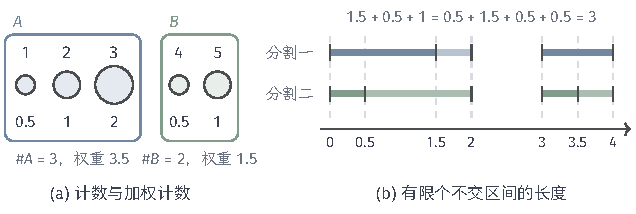
\includegraphics[width=107.6mm]{figures/02-abstract-mathematics/01-metric-and-measure/tikz/c2-count-length/figure.pdf}
  \caption{计数、加权计数与长度遵守同一条不交相加规则。(a)五个点按权重画成大小不同的圆，分成$A=\{1,2,3\}$与$B=\{4,5\}$后，个数$3+2=5$，总权重$3.5+1.5=5$；(b)集合$E=[0,2)\cup[3,4)$的两种不交区间分割，灰色竖线是共同细分的切点，两种分割的长度和都等于$3$。}
  \label{fig:meas-count-length}
\end{figure}

\paragraph{可数拆分时应保持的规则}
上面的可加性只涉及有限个矩形。分析中还会遇到可数拆分。例如
\[
 [0,1)=\bigcup_{k\geq1}\bigl[1-2^{1-k},\,1-2^{-k}\bigr),
\]
这些区间两两不交，长度依次为$\tfrac12,\tfrac14,\tfrac18,\dots$，级数和为$1$，恰好等于$[0,1)$的长度。我们希望这条规则对一切可数拆分都成立：整体长度等于各部分长度的级数和。这不能从有限可加性直接推出，因为有限个区间的拼接只能处理有限个部分。

规则也不能推广到任意多个部分。$[0,1]$是全部单点$\{x\}$之并，每个单点长度为$0$，而“$0$的不可数和”没有定义；若把它理解为$0$，就会得到$[0,1]$的长度为$0$的荒谬结论。所以“有限”与“可数”之间有一条要守住的界线：可数拆分应当保持可加，不可数拆分不作要求。后面建立的测度正是按这条界线设计的。

\subsection{Jordan测量}
\label{sec:meas-jordan}

有限个不交矩形的并只是很少一部分集合。对更一般的有界集合，自然的想法是从里面和外面同时用这类简单集合去逼近，卷二定义区域积分时用的正是这种方法（可参考\BookChapterRef{chap:region-integrals}{卷二第21章“区域积分”}）。下面把有限个有界矩形的并称为\term{初等集合}（elementary set）。它总能改写成有限个不交矩形的并，所以上一小节的体积对它有定义。

\paragraph{内外逼近}
初等集合的体积对包含关系单调。若初等集合$P\subseteq Q$，则$Q\setminus P$仍是初等集合，于是$\lvert P\rvert\leq\lvert P\rvert+\lvert Q\setminus P\rvert=\lvert Q\rvert$。由此可以比较任意一个内部逼近与任意一个外部逼近。

\begin{definition}[Jordan测量]
\label{def:meas-jordan}
设$E\subseteq\mathbb R^d$有界。称
\[
 \begin{aligned}
  J_*(E)&=\sup\{\lvert P\rvert:P\text{为初等集合},\ P\subseteq E\},\\
  J^*(E)&=\inf\{\lvert Q\rvert:Q\text{为初等集合},\ E\subseteq Q\}
 \end{aligned}
\]
分别为$E$的\term{Jordan内测量}（Jordan inner content）与\term{Jordan外测量}（Jordan outer content），其中空集作为初等集合体积为$0$。若$J_*(E)=J^*(E)$，称$E$是\term{Jordan可测}（Jordan measurable）的，公共值记为$J(E)$，称为$E$的\term{Jordan测量}（Jordan content）。
\end{definition}

任取内部初等集合$P\subseteq E$与外部初等集合$Q\supseteq E$，有$P\subseteq Q$，所以$\lvert P\rvert\leq\lvert Q\rvert$，从而总有$J_*(E)\leq J^*(E)$。Jordan可测的意思是两侧能夹逼到同一个数。

\paragraph{边界判据}
两侧逼近之差来自同时接触$E$与$E$外部的那些矩形，所以能否夹逼取决于边界。卷二证明了：有界集合$E$是Jordan可测的，当且仅当它的边界$\partial E$能被有限个总体积任意小的矩形覆盖。直观地说，取一张很细的网格，含于$E$的小块给出内部逼近，与$E$相交的小块给出外部逼近，两者只差与边界相交的小块。

这个判据把问题变成了一个覆盖问题：边界能否用有限个矩形以任意小的总体积盖住。圆盘、多边形等边界光滑或分段光滑的集合都满足它。下面两个一维例子分别说明有限覆盖能做到什么、做不到什么。

\paragraph{有限覆盖可以处理的无限集合}
取$E=\{1/n:n\geq1\}\subseteq\mathbb R$。它不含非退化区间，内测量为$0$。对任意正整数$N$与$\varepsilon>0$，用一个区间$[0,1/N]$盖住$n\geq N$的全部点，再用长度各为$\varepsilon/N$的小区间盖住$1,\tfrac12,\dots,\tfrac1{N-1}$。外部初等集合的总长度不超过$1/N+\varepsilon$，令$N\to\infty$、$\varepsilon\to0$得$J^*(E)=0$。

所以$E$是Jordan可测的，测量为$0$。这里要分清两种“有限”：$E$的元素有无限多个，用来逼近的区间却只有有限个。有限个区间能盖住无限多个点，前提是这些点聚集在少数位置附近；本例中它们聚向$0$，一个短区间就能接住几乎全部的点。

\paragraph{有理点集的反例}
取$E=\mathbb Q\cap[0,1]$。任何非退化区间都含无理数，所以含于$E$的初等集合只能由单点组成，$J_*(E)=0$。另一方面，设初等集合$Q\supseteq E$由区间$I_1,\dots,I_m$组成。把每个$I_k$换成闭包$\overline{I_k}$，长度不变，而$\bigcup_k\overline{I_k}$是含$E$的闭集。$E$在$[0,1]$中稠密，这个闭集必须含$[0,1]$，所以$\lvert Q\rvert\geq1$。$[0,1]$本身是外部初等集合，故$J^*(E)=1$。

内外测量分别为$0$与$1$，$E$不是Jordan可测的。问题出在有限覆盖：有理点到处都是，有限个区间要盖住它们，就不得不连同中间的全部无理数一起盖住。用边界判据看也是一样：$E$的边界是整个$[0,1]$，不能用总长度很小的有限个区间盖住。

\paragraph{改用可数覆盖}
如果允许可数个区间，情况完全不同。把$E$中的点排成一列$q_1,q_2,\dots$。给定$\varepsilon>0$，用长度为$\varepsilon2^{-k}$、以$q_k$为中心的开区间盖住$q_k$。这些区间盖住了$E$，长度总和为$\sum_{k\geq1}\varepsilon2^{-k}=\varepsilon$。图~\ref{fig:meas-jordan-rationals}对比了两种覆盖：有限覆盖必须铺满$[0,1]$，可数覆盖的区间越来越短，总长度可以任意小。在可数覆盖之下，有理点集的大小应当是$0$。

\begin{figure}[!htbp]
  \centering
  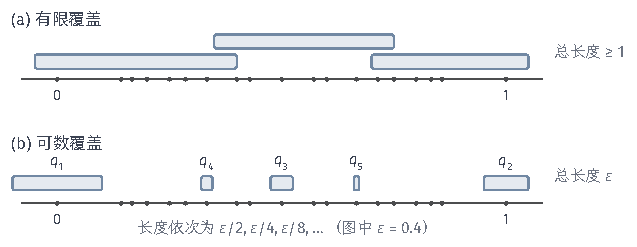
\includegraphics[width=107.8mm]{figures/02-abstract-mathematics/01-metric-and-measure/tikz/c2-jordan-rationals/figure.pdf}
  \caption{用区间覆盖$[0,1]$中的有理点。(a)有限个区间要盖住稠密的有理点，闭包后必须铺满$[0,1]$，总长度不小于$1$；(b)按排列顺序给第$k$个有理点$q_k$分配长度$\varepsilon2^{-k}$的区间，图中只画出前五个，长度依次减半，总长度为$\varepsilon$。}
  \label{fig:meas-jordan-rationals}
\end{figure}

\paragraph{需要重新建立的测量规则}
有理点集还暴露了Jordan测量的另一个缺陷。每个单点都Jordan可测且测量为$0$，它们的可数并$E$却不Jordan可测，所以Jordan可测集合族对可数并不封闭。而分析中处处需要可数运算：一列集合取并或取交，用逐步逼近得到的集合列求极限，把一个集合分成可数个部分。

由此提出两项要求。第一，允许测量的集合族应当对补集和可数并封闭，从而对可数交也封闭。第二，若一个集合被分成可数个不交的可测部分，整体的大小应等于各部分大小的级数和。注意我们没有要求“所有集合都可测”：第一项只规定集合族要有的封闭性，它究竟包含哪些集合，要在构造中确定。下一节先把这两项要求写成定义，满足它们并与长度一致的测量是否存在，由第~\ref{sec:meas-construction}节回答。

\section{测度空间}
\label{sec:meas-measure-spaces}

上一节的两项要求针对两个不同的对象：一项限定哪些集合允许测量，另一项规定怎样给这些集合赋予大小。本节把它们分开建立。

我们先用$\sigma$代数描述允许测量的集合族，并在度量空间上由开集得到Borel集；再在其上定义可数可加的测度，推出比较集合与取极限的规则；最后讨论零测集，说明忽略哪些点不会改变测量，以及怎样把零测集的子集也纳入可测范围。

\subsection{$\sigma$代数}
\label{sec:meas-sigma-algebras}

\paragraph{能够区分哪些集合}
设$X=\{1,2,3,4\}$。若允许测量全部$16$个子集，就能单独询问每个点的大小。若我们只知道每个点属于$\{1,2\}$还是$\{3,4\}$，能够回答的就只有下面四个集合：
\[
 \varnothing,\quad\{1,2\},\quad\{3,4\},\quad X.
\]
单点$\{1\}$这时无法单独测量。两种集合族的底集相同，区分能力不同。

可以把一个集合族看成一份“允许提问的清单”：清单上的集合，才能问它有多大。无论清单选哪一份，都应满足上一节的封闭性要求：能问“在$A$中吗”，就能问“不在$A$中吗”；能问一列集合中的每一个，就能问“至少在其中一个中吗”。把这两条写下来，就是下面的定义。

\begin{definition}[$\sigma$代数]
\label{def:meas-sigma-algebra}
设$X$是集合，$\mathcal A$是$X$的一族子集。若
\begin{enumerate}
 \item $X\in\mathcal A$；
 \item $A\in\mathcal A$蕴含$X\setminus A\in\mathcal A$；
 \item $A_1,A_2,\dots\in\mathcal A$蕴含$\bigcup_{n\geq1}A_n\in\mathcal A$，
\end{enumerate}
则称$\mathcal A$为$X$上的一个\term{$\sigma$代数}（sigma-algebra），称$(X,\mathcal A)$为\term{可测空间}（measurable space），称$\mathcal A$中的集合为\term{可测集合}（measurable set）。
\end{definition}

定义只列出补集与可数并，其他运算由它们得到。由第1、2条，$\varnothing=X\setminus X\in\mathcal A$；在第3条中从某项起全取$\varnothing$，得到有限并封闭。可数交由De Morgan律化为补集与并：
\[
 \bigcap_{n\geq1}A_n=X\setminus\bigcup_{n\geq1}(X\setminus A_n).
\]

差集$A\setminus B=A\cap(X\setminus B)$也属于$\mathcal A$。所以从可测集合出发，经可数次补、并、交、差得到的集合仍然可测。开头的两种清单都满足这些条件：幂集$\mathcal P(X)$含全部子集；四个集合$\varnothing,\{1,2\},\{3,4\},X$中任一个的补集、任意几个的并也都在其中。

\paragraph{生成的$\sigma$代数}
实际问题中，我们通常只点名少数必须能测量的集合，例如区间或若干类别，希望由它们补齐其余集合。给定$X$的一族子集$\mathcal C$，包含$\mathcal C$的$\sigma$代数至少有幂集一个。令$\sigma(\mathcal C)$为所有包含$\mathcal C$的$\sigma$代数之交，称为$\mathcal C$\term{生成的$\sigma$代数}（generated sigma-algebra）。

这个交确实是$\sigma$代数：每个参与求交的$\sigma$代数都含$X$，并对补集、可数并封闭；交集中的元素同时属于它们全体，运算结果也同时属于它们全体。它包含$\mathcal C$，又包含于任何包含$\mathcal C$的$\sigma$代数，所以是其中最小的一个。

这与线性代数中“由一组向量张成的子空间”很像：张成的子空间是包含这组向量的最小子空间，也可以写成所有包含它们的子空间之交。那里的运算是线性组合，这里的运算是补集和可数并。不同之处在于，张成的子空间有“全体有限线性组合”这样的显式表达，而$\sigma(\mathcal C)$一般写不出这样的清单，只能用封闭性来描述。

\begin{example}[有限分组生成的$\sigma$代数]
\label{ex:meas-partition-sigma}
在$X=\{1,2,3,4\}$上取$\mathcal C=\{\{1\},\{2\}\}$。生成的$\sigma$代数必须含$\{1\}$、$\{2\}$，以及
\[
 X\setminus(\{1\}\cup\{2\})=\{3,4\}.
\]
于是它含分组$\{1\},\{2\},\{3,4\}$中任意几组的并，共$2^3=8$个集合。这$8$个集合对补集和并已经封闭，所以它们就是$\sigma(\mathcal C)$，而$\{3\}$不在其中。
\end{example}

图~\ref{fig:meas-partition-sigma}比较了三种分组。有限集合上的$\sigma$代数都由某个分组决定：可测集合恰是若干组之并，组分得越细，可以单独测量的集合就越多。

\begin{BookInlineFigure}
  \centering
  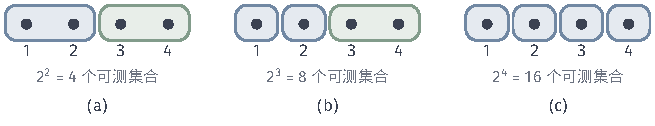
\includegraphics[width=110.938mm]{figures/04-spaces-measures-and-geometry/02-measure/tikz/meas-sigma-algebra-partition/figure.pdf}
  \caption{四点集合$X=\{1,2,3,4\}$上由分组生成的$\sigma$代数。每个色块是一组，可测集合恰是若干组之并。(a)分成$\{1,2\},\{3,4\}$两组；(b)分成$\{1\},\{2\},\{3,4\}$三组；(c)每点自成一组，得到全部子集。}
  \label{fig:meas-partition-sigma}
\end{BookInlineFigure}

生成操作补齐的只是可数运算的封闭性，未必得到所有希望测量的集合。在$\mathbb R$上取全体单点组成的族$\mathcal C$，令$\mathcal D$为可数集合与补集可数的集合的全体。

$\mathcal D$含$\mathbb R$，对补集封闭。对一列$\mathcal D$中的集合，若都可数，则并可数；若其中有一个补集可数，则并的补集包含于它的补集，也可数。所以$\mathcal D$是含全部单点的$\sigma$代数，于是$\sigma(\mathcal C)\subseteq\mathcal D$。

而$[0,1]$与它的补集都不可数，所以$[0,1]\notin\mathcal D$。可见单点生成的$\sigma$代数不含任何非退化区间；要测量区间，生成族里必须直接放入区间或开集。

\paragraph{Borel集}
在度量空间中已经有一族自然的集合：开集。第~\ref{chap:topological-spaces}章用开集表达连续、收敛与紧性，第~\ref{chap:metric-spaces}章又用开球刻画度量空间的开集。把开集作为生成族，得到的可测范围就与这些结构相容。

\begin{definition}[Borel $\sigma$代数]
\label{def:meas-borel}
设$X$是度量空间（更一般地，拓扑空间）。由全体开集生成的$\sigma$代数称为$X$的\term{Borel $\sigma$代数}（Borel sigma-algebra），记作$\mathcal B(X)$，其中的集合称为\term{Borel集}（Borel set）。
\end{definition}

开集的补集是闭集，所以闭集都是Borel集；可数个闭集的并、可数个开集的交也是Borel集。例如$\mathbb Q$是可数个闭集$\{q\}$的并，$[0,1)=\bigcap_{n\geq1}(-1/n,1)$是可数个开集的交，二者都是Borel集。

要强调的是，$\mathcal B(X)$只规定了哪些集合允许测量，并没有规定任何集合的大小。同一个Borel结构上可以放置长度、点质量或它们的组合等不同的测度。

\paragraph{实轴上的生成族}
直接处理全部开集并不方便。下面说明较小的区间族已经够用，关键是把任意开集写成可数个区间的并。

\begin{lemma}[开集的有理区间表示]
\label{lem:meas-open-rational-intervals}
$\mathbb R$中每个开集$U$都是有理端点开区间的可数并。
\end{lemma}

\begin{proof}
任取$x\in U$。因为$U$是开集，存在$r>0$使$(x-r,x+r)\subseteq U$。有理数在实轴上稠密，可取有理数$p,q$满足
\[
 x-r<p<x<q<x+r,
\]
于是$x\in(p,q)\subseteq U$。

所以$U$等于所有含于$U$的有理端点开区间$(p,q)$之并。这样的区间由有序对$(p,q)\in\mathbb Q\times\mathbb Q$确定，而$\mathbb Q\times\mathbb Q$可数，所以这是可数并。
\end{proof}

\begin{theorem}[$\mathcal B(\mathbb R)$的生成族]
\label{thm:meas-borel-generators}
下列每一族集合都生成$\mathcal B(\mathbb R)$：(1)全体开区间$(a,b)$；(2)全体半直线$(a,+\infty)$；(3)全体半直线$(-\infty,a]$；(4)全体左开右闭区间$(a,b]$。在(2)(3)中只取有理数$a$也够用。
\end{theorem}

\begin{proof}
各族中的集合都是开集、闭集或二者之交，属于$\mathcal B(\mathbb R)$，所以它们生成的$\sigma$代数都含于$\mathcal B(\mathbb R)$。反方向只需说明每个开集属于各族生成的$\sigma$代数。对族(1)，这就是引理~\ref{lem:meas-open-rational-intervals}。

其余各族都能经可数运算得到开区间。先看半直线。取有理数列$p_n$严格递减趋于$a$，则
\[
 (a,+\infty)=\bigcup_n(p_n,+\infty),
\]
所以有理端点的半直线已能生成族(2)。又因$(-\infty,a]$的补集是$(a,+\infty)$，族(3)与族(2)生成同一个$\sigma$代数。

再看半开区间与开区间。由下面两个等式：
\[
 (a,b]=(-\infty,b]\setminus(-\infty,a],\qquad
 (a,b)=\bigcup_{n}\,(a,\,b-1/n]
\]
（后式中$n$取使$b-1/n>a$的整数），可知开区间属于族(3)或族(4)生成的$\sigma$代数。
\end{proof}

同样的论证在$\mathbb R^d$中成立：每个开集是可数个有理顶点开矩形之并，所以开矩形生成$\mathcal B(\mathbb R^d)$；把开矩形写成左开右闭矩形的可数并，可知左开右闭矩形$\prod_i(a_i,b_i]$也生成$\mathcal B(\mathbb R^d)$。

\subsection{测度及其基本性质}
\label{sec:meas-measures}

\paragraph{测度的定义}
可测范围确定以后，要给每个可测集合配一个非负的大小，并要求可数可加。允许取值$+\infty$，因为整条实轴的长度、无限集合的元素个数都没有有限的值。在$[0,+\infty]$中约定$a+(+\infty)=+\infty$，非负项级数的和是部分和的上确界，可以为$+\infty$。

\begin{definition}[测度]
\label{def:meas-measure}
设$(X,\mathcal A)$是可测空间。映射$\mu:\mathcal A\to[0,+\infty]$若满足$\mu(\varnothing)=0$，并且对两两不交的$A_1,A_2,\dots\in\mathcal A$有
\begin{equation}
 \mu\Bigl(\bigcup_{n\geq1}A_n\Bigr)=\sum_{n\geq1}\mu(A_n),
 \label{eq:meas-countable-additivity}
\end{equation}
则称$\mu$为$(X,\mathcal A)$上的\term{测度}（measure），称$(X,\mathcal A,\mu)$为\term{测度空间}（measure space）。式~\eqref{eq:meas-countable-additivity}称为\term{可数可加性}（countable additivity）。
\end{definition}

非负项级数的和与求和次序无关，所以式~\eqref{eq:meas-countable-additivity}右端不依赖集合的排列方式，这与左端的并集不依赖排列相一致。条件$\mu(\varnothing)=0$排除了一切集合都取$+\infty$的平凡赋值；若某个$A$满足$\mu(A)<+\infty$，取$A_1=A$、其余为空集，由式~\eqref{eq:meas-countable-additivity}也能推出它。

\paragraph{计数测度与点质量}
在任意可测空间上，令$\mu(A)=\#A$（$A$为无限集时取$+\infty$），称为\term{计数测度}（counting measure）。核对可数可加性：若不交的$A_n$中只有有限个非空且都是有限集，两边都是元素总数；若某个$A_n$无限，或有无限多个$A_n$非空，并集无限，右边的级数也发散到$+\infty$。

固定$x\in X$，规定
\[
 \delta_x(A)=\begin{cases}1,&x\in A,\\0,&x\notin A,\end{cases}
\]
称为点$x$处的\term{Dirac测度}（Dirac measure）。不交集合列中至多一个含$x$，所以可数可加性成立。

这个定义只读取可测集合$A$是否含$x$，并不要求单点$\{x\}$本身可测。例如在$\mathcal A=\{\varnothing,\{1,2\},\{3,4\},X\}$上，$\delta_1$给$\{1,2\}$赋值$1$，给$\{3,4\}$赋值$0$，尽管$\{1\}$不可测。

把可数个点质量按非负权重相加，得到$\mu=\sum_kw_k\delta_{x_k}$，即$\mu(A)=\sum_{k:x_k\in A}w_k$。它推广了上一节的加权计数。核对可数可加性时要交换两重求和：
\[
 \sum_n\sum_kw_k\delta_{x_k}(A_n)=\sum_k\sum_nw_k\delta_{x_k}(A_n).
\]
非负二重级数的两种累次求和相等，因为任意有限部分和都不超过另一种次序的总和，令有限范围扩大即得两个方向的不等式。

例如在$\mathbb N=\{1,2,\dots\}$上取$\mu=\sum_n2^{-n}\delta_n$。总量是
\[
 \mu(\mathbb N)=\sum_{n\geq1}2^{-n}=1,
\]
偶数集的测度是
\[
 \mu(\{2,4,6,\dots\})=\sum_{m\geq1}2^{-2m}=\sum_{m\geq1}4^{-m}=\frac13.
\]

\paragraph{有限性条件}
测度可以整体取$+\infty$，但不同测度“无限”的方式差别很大，后面一些结论要区分它们。

\begin{definition}[有限测度、概率测度与$\sigma$有限测度]
\label{def:meas-finiteness}
设$(X,\mathcal A,\mu)$是测度空间。若$\mu(X)<+\infty$，称$\mu$为\term{有限测度}（finite measure）；若$\mu(X)=1$，称$\mu$为\term{概率测度}（probability measure）；若存在$X_1,X_2,\dots\in\mathcal A$使$X=\bigcup_nX_n$且每个$\mu(X_n)<+\infty$，称$\mu$为\term{$\sigma$有限测度}（sigma-finite measure）。
\end{definition}

有限测度都是$\sigma$有限的。$\mathbb N$上的计数测度总量为$+\infty$，但$\mathbb N=\bigcup_n\{n\}$且每个单点计数为$1$，所以它$\sigma$有限：整体无限，却能切成可数个有限的片。

$\mathbb R$上以全部子集为可测范围的计数测度不是$\sigma$有限的。若$\mathbb R=\bigcup_nX_n$且每个$X_n$都是有限集，$\mathbb R$就可数了，这是矛盾。唯一性定理和乘积测度需要$\sigma$有限条件，下面的基本性质不需要；我们在每处单独声明，不把它当作统一假设。

\paragraph{基本性质}
可数可加性只直接说到不交集合。比较有包含关系的集合、处理互相重叠的集合、对集合列取极限，都要先把集合拆成不交的部分。

\begin{theorem}[测度的基本性质]
\label{thm:meas-basic-properties}
设$(X,\mathcal A,\mu)$是测度空间，以下集合都属于$\mathcal A$。
\begin{enumerate}
 \item 有限可加性：若$A_1,\dots,A_m$两两不交，则
 \begin{equation}
  \mu\Bigl(\bigcup_{k=1}^mA_k\Bigr)=\sum_{k=1}^m\mu(A_k).
  \label{eq:meas-finite-additive}
 \end{equation}
 \item 单调性：$A\subseteq B$蕴含$\mu(A)\leq\mu(B)$；若还有$\mu(A)<+\infty$，则
 \begin{equation}
  \mu(B\setminus A)=\mu(B)-\mu(A).
  \label{eq:meas-monotone-difference}
 \end{equation}
 \item 可数次可加性：$A_n$不必两两不交，都有
 \begin{equation}
  \mu\Bigl(\bigcup_nA_n\Bigr)\leq\sum_n\mu(A_n).
  \label{eq:meas-countable-subadditive}
 \end{equation}
 \item 从下连续性：若$A_1\subseteq A_2\subseteq\cdots$，则
 \begin{equation}
  \mu\Bigl(\bigcup_nA_n\Bigr)=\lim_{n\to\infty}\mu(A_n).
  \label{eq:meas-continuity-below}
 \end{equation}
 \item 从上连续性：若$A_1\supseteq A_2\supseteq\cdots$且$\mu(A_1)<+\infty$，则
 \begin{equation}
  \mu\Bigl(\bigcap_nA_n\Bigr)=\lim_{n\to\infty}\mu(A_n).
  \label{eq:meas-continuity-above}
 \end{equation}
\end{enumerate}
\end{theorem}

\begin{proof}
第1条在可数可加性中令$A_n=\varnothing$（$n>m$）即得。

对第2条，$B=A\cup(B\setminus A)$是不交并，由第1条
\[
 \mu(B)=\mu(A)+\mu(B\setminus A)\geq\mu(A).
\]
当$\mu(A)$有限时，两边可以减去$\mu(A)$，得到差集的公式。

对第3条，先把重叠的部分去掉：令$B_1=A_1$，$B_n=A_n\setminus\bigcup_{k<n}A_k$。这些$B_n$两两不交，$B_n\subseteq A_n$，并且$\bigcup_nB_n=\bigcup_nA_n$。由可数可加性与单调性，
\[
 \mu\Bigl(\bigcup_nA_n\Bigr)=\sum_n\mu(B_n)\leq\sum_n\mu(A_n).
\]

对第4条，令$A_0=\varnothing$，$D_n=A_n\setminus A_{n-1}$。这些相邻差集两两不交，$A_n=\bigcup_{k\leq n}D_k$，$\bigcup_nA_n=\bigcup_kD_k$，所以
\[
 \mu\Bigl(\bigcup_nA_n\Bigr)=\sum_{k=1}^{\infty}\mu(D_k)
 =\lim_{n\to\infty}\sum_{k=1}^n\mu(D_k)=\lim_{n\to\infty}\mu(A_n).
\]

对第5条，令$C_n=A_1\setminus A_n$，它们递增，并为$A_1\setminus\bigcap_nA_n$。由第4条，
\[
 \mu\Bigl(A_1\setminus\bigcap_nA_n\Bigr)=\lim_{n\to\infty}\mu(A_1\setminus A_n).
\]
因为$\mu(A_1)<+\infty$，第2条允许把两边写成差：
\[
 \mu(A_1)-\mu\Bigl(\bigcap_nA_n\Bigr)=\mu(A_1)-\lim_{n\to\infty}\mu(A_n).
\]
消去有限数$\mu(A_1)$，即得结论。
\end{proof}

这两条连续性可以用同一个测度手算。在$\mathbb N$上取$\mu=\sum_n2^{-n}\delta_n$，令递增列$A_n=\{1,\dots,n\}$，递减列$B_n=\{n,n+1,\dots\}$。则
\[
 \mu(A_n)=1-2^{-n}\to1=\mu(\mathbb N),\qquad
 \mu(B_n)=2^{1-n}\to0=\mu(\varnothing).
\]
递增时测度从下面爬向极限集合的测度，递减时测度从上面落到极限集合的测度，两者都正好对上式~\eqref{eq:meas-continuity-below}与式~\eqref{eq:meas-continuity-above}。

第5条中的有限性条件不能省略。在$\mathbb N$上取计数测度与尾集$A_n=\{n,n+1,\dots\}$。每个$A_n$都是无限集，$\mu(A_n)=+\infty$，而$\bigcap_nA_n=\varnothing$，测度为$0$。证明失效的位置是“两边减去$\mu(A_1)$”，因为$+\infty-(+\infty)$没有意义。

只要从某项起$\mu(A_n)$有限，把这一项当作首项即可应用第5条。所以从下连续性无条件成立，从上连续性需要一个有限的起点，两者不能混用。

\paragraph{限制与加权和}
从已有测度得到新测度有几种常用操作。设$E\in\mathcal A$，令$\mu|_E(A)=\mu(A\cap E)$，它仍是$(X,\mathcal A)$上的测度，只保留$E$内的质量。

若$\mu_1,\mu_2,\dots$是测度，$c_k\in[0,+\infty]$，并约定$0\cdot(+\infty)=0$，则$\sum_kc_k\mu_k$也是测度；核对可数可加性时同样只需交换非负二重级数的求和次序。约定$0\cdot(+\infty)=0$保证系数为零的项对任何集合都贡献零，不会产生没有定义的乘积。

\subsection{测度的完备化}
\label{sec:meas-completion}

\paragraph{零测集与几乎处处}
测量中常有一些例外点：它们存在，但质量为零，不影响任何集合的大小。我们希望能说“除去一个可以忽略的集合，某性质成立”。

\begin{definition}[零测集与几乎处处]
\label{def:meas-null-set}
设$(X,\mathcal A,\mu)$是测度空间。满足$\mu(N)=0$的$N\in\mathcal A$称为$\mu$-\term{零测集}（null set）。若使某个关于点的性质不成立的点全体包含于某个$\mu$-零测集，称该性质$\mu$-\term{几乎处处}（almost everywhere）成立，记作$\mu$-a.e.。
\end{definition}

“逐点成立”要求性质在每一点都对，“几乎处处成立”允许它在一个零测集上失败。定义只要求失败点集\emph{包含于}一个零测集，因为失败点集本身未必可测。

几乎处处总是相对于当前测度而言的。在$X=\{0,1\}$与$\mathcal A=\mathcal P(X)$上，$\{1\}$是$\delta_0$的零测集，却承载$\delta_1$的全部质量。于是“函数在点$1$以外取零”对$\delta_0$几乎处处成立，对$\delta_1$不成立，这句话换一个测度就要重新判断。

可数个零测例外可以合并：若$N_1,N_2,\dots$都是零测集，由可数次可加性，
\[
 \mu\Bigl(\bigcup_nN_n\Bigr)\leq\sum_n\mu(N_n)=0.
\]
所以一列性质若各自几乎处处成立，它们同时几乎处处成立。这一论证依赖可数次可加性，对不可数个零测集不适用；下一节构造长度测度后会看到，$[0,1]$是不可数个长度为零的单点之并，自身长度却为$1$。

\paragraph{零测集的子集}
零测集的子集“更应当”可以忽略，可它不一定可测。在$X=\{1,2,3\}$上取$\mathcal A=\{\varnothing,\{1\},\{2,3\},X\}$与$\mu=\delta_1$，$\{2,3\}$是零测集，它的子集$\{2\}$却不可测，连“$\{2\}$的测度为零”这句话都说不出。

\begin{definition}[完备测度空间]
\label{def:meas-complete}
若测度空间$(X,\mathcal A,\mu)$中每个零测集的每个子集都属于$\mathcal A$，称该测度空间是\term{完备}（complete）的。
\end{definition}

这里的完备与第~\ref{chap:metric-spaces}章度量空间的完备性（Cauchy列收敛）是两个不同的概念，只是同名。不完备的测度空间可以通过补入零测集的子集来修补，关键是补入以后不能改变原有集合的测度。

\begin{theorem}[测度空间的完备化]
\label{thm:meas-completion}
设$(X,\mathcal A,\mu)$是测度空间。令$\overline{\mathcal A}$为形如$A\cup M$的集合全体，其中$A\in\mathcal A$，$M$包含于某个$\mu$-零测集；规定$\overline\mu(A\cup M)=\mu(A)$。则$\overline{\mathcal A}$是包含$\mathcal A$的$\sigma$代数，$\overline\mu$是其上不依赖表示方式的测度，在$\mathcal A$上与$\mu$一致，且$(X,\overline{\mathcal A},\overline\mu)$完备。它称为$(X,\mathcal A,\mu)$的\term{完备化}（completion）。
\end{theorem}

\begin{proof}
先证赋值与表示方式无关。设$A\cup M=A'\cup M'$，其中$M\subseteq N$、$M'\subseteq N'$，$N,N'$是零测集。则$A\subseteq A'\cup N'$，由单调性与次可加性，
\[
 \mu(A)\leq\mu(A')+\mu(N')=\mu(A').
\]
对称地$\mu(A')\leq\mu(A)$，所以$\mu(A)=\mu(A')$。取$M=\varnothing$可知$\mathcal A\subseteq\overline{\mathcal A}$，且$\overline\mu$在$\mathcal A$上等于$\mu$。

再证$\overline{\mathcal A}$是$\sigma$代数。对补集，设$M\subseteq N$，则
\[
 X\setminus(A\cup M)=\bigl((X\setminus A)\setminus N\bigr)\cup\bigl((X\setminus A)\cap(N\setminus M)\bigr),
\]
第一项属于$\mathcal A$，第二项包含于零测集$N$。对可数并，
\[
 \bigcup_n(A_n\cup M_n)=\Bigl(\bigcup_nA_n\Bigr)\cup\Bigl(\bigcup_nM_n\Bigr),
\]
而$\bigcup_nM_n\subseteq\bigcup_nN_n$，后者是零测集。

然后证可数可加性。若$A_n\cup M_n$两两不交，则$A_n$两两不交，于是
\[
 \overline\mu\Bigl(\bigcup_n(A_n\cup M_n)\Bigr)=\mu\Bigl(\bigcup_nA_n\Bigr)
 =\sum_n\mu(A_n)=\sum_n\overline\mu(A_n\cup M_n).
\]

最后证完备性。若$\overline\mu(A\cup M)=0$，则$\mu(A)=0$，$A\cup M\subseteq A\cup N$，后者是$\mu$-零测集。$A\cup M$的任一子集$S$可写成$\varnothing\cup S$，其中$S$包含于零测集$A\cup N$，所以$S\in\overline{\mathcal A}$。
\end{proof}

在上面的例子中，零测集$\{2,3\}$的子集$\{2\}$、$\{3\}$被补入，得到$\overline{\mathcal A}=\mathcal P(X)$，$\overline\mu=\delta_1$。完备化不改变原有集合的测度，只把“包含于零测集”的集合也纳入可测范围并赋值为零。

是否需要完备化取决于问题：讨论零测集上修改函数后的可测性时它很方便，讨论乘积空间的截面时它又会带来额外的例外，这一点在第~\ref{chap:integration}章再说明。

\section{测度的构造}
\label{sec:meas-construction}

上一节规定了测度应满足的规则，并用计数、点质量等例子验证了这些规则可以实现。可是第~\ref{sec:meas-size-additivity}节真正想要的长度测度还没有出现：我们只知道区间的长度，并不知道怎样把它可数可加地推广到$\mathcal B(\mathbb R)$。

本节分三步回答。先把可数覆盖的想法做成外测度，从中选出满足分割可加的集合；再把这条路线抽象成从简单集合族出发的延拓定理，分别回答延拓是否存在、是否唯一；最后用它构造实轴上的Lebesgue测度和Stieltjes测度。

\subsection{外测度}
\label{sec:meas-outer-measure}

\paragraph{覆盖的总费用}
有理点集的例子提示了一种测量方式：用一列简单集合覆盖待测集合，算出覆盖的总费用，再让总费用尽量小。可以把简单集合想成一种按件定价的“包装”，给一个集合算大小，就是问把它完全打包最少要花多少钱。这样得到的量对每个子集都有定义，但它满足的规则比测度少。

\begin{definition}[外测度]
\label{def:meas-outer}
集合$X$上的\term{外测度}（outer measure）是映射$\mu^*:\mathcal P(X)\to[0,+\infty]$，满足：$\mu^*(\varnothing)=0$；$E\subseteq F$蕴含$\mu^*(E)\leq\mu^*(F)$；对任意$E_1,E_2,\dots\subseteq X$，有
\begin{equation}
 \mu^*\Bigl(\bigcup_nE_n\Bigr)\leq\sum_n\mu^*(E_n).
 \label{eq:meas-outer-subadditive}
\end{equation}
\end{definition}

外测度只要求次可加，不要求可加。下面的引理说明，任何一种“简单集合的费用”都能经可数覆盖变成外测度，这就是把局部赋值推广到任意子集的方法。

\begin{lemma}[由覆盖得到外测度]
\label{lem:meas-cover-outer}
设$\mathcal C$是$X$的一族子集，$\varnothing\in\mathcal C$，$\rho:\mathcal C\to[0,+\infty]$满足$\rho(\varnothing)=0$。对$E\subseteq X$令
\begin{equation}
 \mu^*(E)=\inf\Bigl\{\sum_{n\geq1}\rho(C_n):C_n\in\mathcal C,\ E\subseteq\bigcup_{n\geq1}C_n\Bigr\},
 \label{eq:meas-cover-outer}
\end{equation}
没有这样的覆盖时取$+\infty$。则$\mu^*$是外测度。
\end{lemma}

\begin{proof}
取全部$C_n=\varnothing$覆盖空集，得$\mu^*(\varnothing)=0$。若$E\subseteq F$，覆盖$F$的每一列集合也覆盖$E$，下确界取在更大的范围上，故$\mu^*(E)\leq\mu^*(F)$。

对次可加性，不妨设$\sum_n\mu^*(E_n)<+\infty$，任取$\varepsilon>0$。对每个$n$，按下确界的定义选覆盖$E_n$的$C_{n,1},C_{n,2},\dots\in\mathcal C$，使
\[
 \sum_k\rho(C_{n,k})\leq\mu^*(E_n)+\varepsilon2^{-n}.
\]

全体$C_{n,k}$可以排成一列并覆盖$\bigcup_nE_n$，非负项的排列不改变级数和，于是
\[
 \mu^*\Bigl(\bigcup_nE_n\Bigr)\leq\sum_n\sum_k\rho(C_{n,k})
 \leq\sum_n\bigl(\mu^*(E_n)+\varepsilon2^{-n}\bigr)=\sum_n\mu^*(E_n)+\varepsilon.
\]
令$\varepsilon\to0$即得结论。
\end{proof}

外测度能给每个子集赋值，代价是失去可加性。在$X=\{1,2\}$上取$\mathcal C=\{\varnothing,X\}$、$\rho(X)=1$。唯一有效的覆盖是$X$本身，所以
\[
 \mu^*(\{1\})=\mu^*(\{2\})=\mu^*(X)=1.
\]
不交的$\{1\}$与$\{2\}$外测度之和为$2$，它们的并的外测度却是$1$。原因是这份价目表只卖整包，无法把两点分开计价，见图~\ref{fig:meas-carath-cut}(b)。因此要找出外测度在哪些集合上可加。

\paragraph{Carathéodory可测性}
一个集合$A$要“与外测度相容”，应当意味着用$A$去切任何集合都不会多算或少算。图~\ref{fig:meas-carath-cut}(a)画的正是这个检验：拿一个测试集合$E$，用$A$切成两块，比较切开前后的总价。只在一个特定的$E$上检验还不够，下面的判据要求对一切测试集合都成立。

\begin{BookInlineFigure}
  \centering
  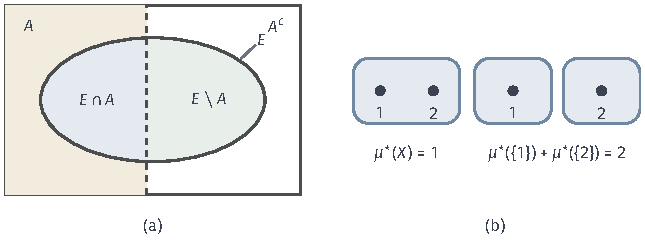
\includegraphics[width=109.238mm]{figures/04-spaces-measures-and-geometry/02-measure/tikz/meas-carath-cut/figure.pdf}
  \caption{Carathéodory判据的含义。(a)测试集合$E$（椭圆）被$A$切成$E\cap A$（蓝）与$E\setminus A$（绿），可测要求两块的外测度之和总等于$\mu^*(E)$；(b)价目表只卖整包$X$时，切开$X=\{1,2\}$迫使每点各付一个整包的价，$\{1\}$不满足判据。}
  \label{fig:meas-carath-cut}
\end{BookInlineFigure}

\begin{definition}[Carathéodory可测]
\label{def:meas-caratheodory-measurable}
设$\mu^*$是$X$上的外测度。若对每个$E\subseteq X$都有
\begin{equation}
 \mu^*(E)=\mu^*(E\cap A)+\mu^*(E\setminus A),
 \label{eq:meas-caratheodory-criterion}
\end{equation}
称$A\subseteq X$为$\mu^*$-\term{Carathéodory可测}（Carathéodory measurable）的。
\end{definition}

由次可加性，“$\leq$”总成立，所以验证时只需证明“$\geq$”，并且只需对$\mu^*(E)<+\infty$的$E$验证。上例中$\{1\}$不满足判据：取$E=X$，右边为$2$，左边为$1$。

再看一个能选出非平凡集合的例子。取$X=\{1,2,3\}$，价目表$\mathcal C=\{\varnothing,\{1\},\{2,3\},X\}$，价格为
\[
 \rho(\{1\})=1,\qquad\rho(\{2,3\})=2,\qquad\rho(X)=3.
\]
点$2$、$3$只能打包购买。由式~\eqref{eq:meas-cover-outer}，单点和两点集的外测度是
\[
 \mu^*(\{1\})=1,\quad \mu^*(\{2\})=\mu^*(\{3\})=\mu^*(\{2,3\})=2,\quad \mu^*(\{1,2\})=3.
\]

检验$A=\{1\}$：取$E=X$，$1+2=3$；取$E=\{2\}$，$0+2=2$；取$E=\{1,2\}$，$1+2=3$，等式都成立，其余$E$同样核对。检验$A=\{2\}$：取$E=\{2,3\}$，右边是$\mu^*(\{2\})+\mu^*(\{3\})=4$，左边是$2$，判据不成立。

逐一检查可知全部可测集是$\varnothing,\{1\},\{2,3\},X$：恰好是价目表上明码标价的那些集合。下面的定理说明，这样选出的集合总是构成$\sigma$代数，外测度在上面可数可加。

\begin{theorem}[Carathéodory定理]
\label{thm:meas-caratheodory}
设$\mu^*$是$X$上的外测度，$\mathcal M$为全体$\mu^*$-Carathéodory可测集。则$\mathcal M$是$\sigma$代数，$\mu^*$在$\mathcal M$上的限制是测度，且$(X,\mathcal M,\mu^*|_{\mathcal M})$完备；特别地，$\mu^*(N)=0$的集合$N$都属于$\mathcal M$。
\end{theorem}

证明分三步：先处理补集与有限并，再控制可数不交并，最后由不交化得到一般的可数并，同时读出可数可加性。

\begin{proof}
\emph{补集与有限并。}判据关于$A$与$X\setminus A$对称，所以$\mathcal M$对补集封闭；$X\in\mathcal M$是因为$\mu^*(\varnothing)=0$。

设$A,B\in\mathcal M$，$E\subseteq X$。先用$A$切$E$，再用$B$切$E\setminus A$，得到
\[
 \mu^*(E)=\mu^*(E\cap A)+\mu^*\bigl((E\setminus A)\cap B\bigr)+\mu^*\bigl(E\setminus(A\cup B)\bigr).
\]
把前两项涉及的两块并起来，就是$A\cup B$切出的部分：
\[
 E\cap(A\cup B)=(E\cap A)\cup\bigl((E\setminus A)\cap B\bigr).
\]
次可加性说明前两项之和不小于$\mu^*(E\cap(A\cup B))$，于是
\[
 \mu^*(E)\geq\mu^*\bigl(E\cap(A\cup B)\bigr)+\mu^*\bigl(E\setminus(A\cup B)\bigr).
\]
这就是$A\cup B$的判据。于是$\mathcal M$对有限并、有限交与差都封闭。

\emph{可数不交并。}设$A_1,A_2,\dots\in\mathcal M$两两不交，$B_n=\bigcup_{k\leq n}A_k$，$B=\bigcup_kA_k$。用$A_n$切测试集合$E\cap B_n$，因$A_n$与$B_{n-1}$不交，得
\[
 \mu^*(E\cap B_n)=\mu^*(E\cap A_n)+\mu^*(E\cap B_{n-1}).
\]
对$n$归纳，得到
\[
 \mu^*(E\cap B_n)=\sum_{k\leq n}\mu^*(E\cap A_k).
\]

再用$B_n\in\mathcal M$切$E$，并由$E\setminus B_n\supseteq E\setminus B$及单调性，得
\[
 \mu^*(E)=\mu^*(E\cap B_n)+\mu^*(E\setminus B_n)
 \geq\sum_{k\leq n}\mu^*(E\cap A_k)+\mu^*(E\setminus B).
\]
令$n\to\infty$，再用次可加性，
\begin{equation}
 \mu^*(E)\geq\sum_{k\geq1}\mu^*(E\cap A_k)+\mu^*(E\setminus B)
 \geq\mu^*(E\cap B)+\mu^*(E\setminus B).
 \label{eq:meas-caratheodory-chain}
\end{equation}
所以$B\in\mathcal M$。在式~\eqref{eq:meas-caratheodory-chain}中取$E=B$，得$\mu^*(B)\geq\sum_k\mu^*(A_k)$，与次可加性合起来就是$\mu^*(B)=\sum_k\mu^*(A_k)$。

\emph{一般可数并与零外测度集。}对任意$A_n\in\mathcal M$，令$A'_n=A_n\setminus\bigcup_{k<n}A_k$。它们属于$\mathcal M$且两两不交，$\bigcup_nA'_n=\bigcup_nA_n$，由上一步知后者属于$\mathcal M$。因此$\mathcal M$是$\sigma$代数，$\mu^*$在其上可数可加。

若$\mu^*(N)=0$，则对任意$E$，由单调性，
\[
 \mu^*(E\cap N)+\mu^*(E\setminus N)\leq0+\mu^*(E),
\]
故$N\in\mathcal M$。零测集的子集外测度也为零，所以属于$\mathcal M$，测度空间完备。
\end{proof}

定理只保证$\mathcal M$是$\sigma$代数，并不保证它含有我们关心的集合；在第一个例子中，$\mathcal M=\{\varnothing,X\}$。对具体的外测度，还要验证想测量的集合（例如区间）满足判据。下一小节说明，只要初始赋值本身可数可加，这一步总能完成。

\subsection{测度延拓}
\label{sec:meas-extension}

\paragraph{集合代数与预测度}
Lebesgue测度的构造可以抽象出来：先在一族简单集合上给出赋值，再用覆盖得到外测度，最后由Carathéodory定理得到$\sigma$代数上的测度。这族简单集合只需对有限运算封闭，赋值则必须在“并集恰好仍是简单集合”的范围内可数可加。

\begin{definition}[集合代数与预测度]
\label{def:meas-algebra-premeasure}
$X$的一族子集$\mathcal R$若含$X$，并对补集和有限并封闭，称为$X$上的\term{集合代数}（algebra of sets）。映射$\mu_0:\mathcal R\to[0,+\infty]$若满足$\mu_0(\varnothing)=0$，并且对两两不交、并集仍属于$\mathcal R$的$A_1,A_2,\dots\in\mathcal R$有
\begin{equation}
 \mu_0\Bigl(\bigcup_nA_n\Bigr)=\sum_n\mu_0(A_n),
 \label{eq:meas-premeasure-additivity}
\end{equation}
称为$\mathcal R$上的\term{预测度}（premeasure）。若存在$X_n\in\mathcal R$使$X=\bigcup_nX_n$且$\mu_0(X_n)<+\infty$，称$\mu_0$是$\sigma$有限的。
\end{definition}

集合代数只保证有限运算的结果仍在其中，可数并可能跑出去，所以预测度的可数可加性只在并集仍属于$\mathcal R$时提出。实践中常从更小的半环出发，例如$\mathbb R$中全体$(a,b]$；它们的有限不交并组成一个集合代数，先把赋值按不交分块相加扩展到这个代数上，再使用下面的定理。

\paragraph{有限可加不够}
预测度的条件不能减弱为有限可加。在$\mathbb N$上取$\mathcal R$为有限集与补集有限的集合全体，它是集合代数。令$\mu_0(A)=0$（$A$有限）或$1$（$A$的补集有限）。两个不交集合不可能都补集有限，所以$\mu_0$有限可加。

但$\mathbb N=\bigcup_n\{n\}$是$\mathcal R$中不交集合的可数并，并且$\mathbb N\in\mathcal R$，式~\eqref{eq:meas-premeasure-additivity}两边分别是$1$和$0$。这个赋值不是预测度，也不可能延拓为$\sigma(\mathcal R)=\mathcal P(\mathbb N)$上的测度，因为任何测度都必须满足这条可数可加的等式。

\paragraph{延拓的存在性}
预测度正是使覆盖构造成功的条件：它保证外测度在简单集合上不改变原赋值，并使这些集合通过Carathéodory判据。

\begin{theorem}[延拓的存在性]
\label{thm:meas-extension-existence}
设$\mu_0$是集合代数$\mathcal R$上的预测度，按式~\eqref{eq:meas-cover-outer}用$\mathcal R$中集合的可数覆盖定义外测度$\mu^*$。则$\mu^*(A)=\mu_0(A)$对$A\in\mathcal R$成立，并且$\mathcal R$中的集合都是$\mu^*$-Carathéodory可测的。因此$\mu^*$限制在$\sigma(\mathcal R)$上是延拓$\mu_0$的测度。
\end{theorem}

\begin{proof}
先证$\mu^*=\mu_0$在$\mathcal R$上成立。$A$本身覆盖$A$，故$\mu^*(A)\leq\mu_0(A)$。

反方向，设$C_n\in\mathcal R$覆盖$A$，令$D_n=(A\cap C_n)\setminus\bigcup_{k<n}C_k$。这些集合属于$\mathcal R$，两两不交，并集为$A\in\mathcal R$。由预测度的可数可加性，以及有限可加性推出的单调性，
\[
 \mu_0(A)=\sum_n\mu_0(D_n)\leq\sum_n\mu_0(C_n).
\]
对覆盖取下确界，得$\mu_0(A)\leq\mu^*(A)$。

再证$A\in\mathcal R$满足判据。设$\mu^*(E)<+\infty$，$\varepsilon>0$，取$C_n\in\mathcal R$覆盖$E$且$\sum_n\mu_0(C_n)\leq\mu^*(E)+\varepsilon$。集合$C_n\cap A$与$C_n\setminus A$属于$\mathcal R$，分别覆盖$E\cap A$与$E\setminus A$，并且$\mu_0(C_n)=\mu_0(C_n\cap A)+\mu_0(C_n\setminus A)$。于是
\[
\begin{aligned}
 \mu^*(E\cap A)+\mu^*(E\setminus A)
 &\leq\sum_n\mu_0(C_n\cap A)+\sum_n\mu_0(C_n\setminus A)\\
 &=\sum_n\mu_0(C_n)\leq\mu^*(E)+\varepsilon.
\end{aligned}
\]
令$\varepsilon\to0$，得到判据。

由Carathéodory定理，可测集构成含$\mathcal R$的$\sigma$代数，所以含$\sigma(\mathcal R)$，$\mu^*$在其上是测度并延拓$\mu_0$。
\end{proof}

\paragraph{$\pi$系统与$\lambda$系统}
唯一性要说明：两个测度若在$\mathcal R$上相等，则在$\sigma(\mathcal R)$上相等。自然的做法是考察“两测度取值相等的集合”构成的族$\mathcal D$，希望它是含$\mathcal R$的$\sigma$代数。

可是$\mathcal D$只对补集和不交可数并封闭，对一般的并未必封闭，因为$\mu(A\cup B)=\mu(A)+\mu(B)-\mu(A\cap B)$要求先知道交集上的取值。这启发我们把封闭性要求拆成两部分。

\begin{definition}[$\pi$系统与$\lambda$系统]
\label{def:meas-pi-lambda-systems}
$X$的一族子集$\mathcal P$若对有限交封闭，称为\term{$\pi$系统}（pi-system）。一族子集$\mathcal D$若含$X$，对补集封闭，并对两两不交的可数并封闭，称为\term{$\lambda$系统}（lambda-system）。
\end{definition}

$\sigma$代数既是$\pi$系统又是$\lambda$系统。反过来，若一族集合同时是二者，它对有限交、补集封闭，从而对有限并封闭。对一般可数并，不交化
\[
 A_n\setminus\bigcup_{k<n}A_k=A_n\cap\bigcap_{k<n}(X\setminus A_k)
\]
只用到有限交与补集，所以这族集合是$\sigma$代数。

\begin{theorem}[$\pi$--$\lambda$定理]
\label{thm:meas-pi-lambda}
若$\pi$系统$\mathcal P$包含于$\lambda$系统$\mathcal D$，则$\sigma(\mathcal P)\subseteq\mathcal D$。
\end{theorem}

\begin{proof}
令$\ell(\mathcal P)$为所有包含$\mathcal P$的$\lambda$系统之交，它仍是$\lambda$系统，且$\ell(\mathcal P)\subseteq\mathcal D$。由上一段，只需证明$\ell(\mathcal P)$对有限交封闭，那时它是含$\mathcal P$的$\sigma$代数，于是$\sigma(\mathcal P)\subseteq\ell(\mathcal P)\subseteq\mathcal D$。

对集合$A\in\ell(\mathcal P)$，令$\mathcal D_A=\{B:A\cap B\in\ell(\mathcal P)\}$。它是$\lambda$系统，逐条核对如下。首先$X\in\mathcal D_A$。其次，若$B\in\mathcal D_A$，则
\[
 A\cap(X\setminus B)=X\setminus\bigl((X\setminus A)\cup(A\cap B)\bigr),
\]
括号内是$\ell(\mathcal P)$中两个不交集合之并，所以属于$\ell(\mathcal P)$，取补集仍属于$\ell(\mathcal P)$。最后，若$B_n\in\mathcal D_A$两两不交，则$A\cap\bigcup_nB_n=\bigcup_n(A\cap B_n)$是$\ell(\mathcal P)$中不交集合的可数并。

先取$A\in\mathcal P$。$\mathcal P$对交封闭，所以$\mathcal P\subseteq\mathcal D_A$，由最小性$\ell(\mathcal P)\subseteq\mathcal D_A$。这说明$A\cap B\in\ell(\mathcal P)$对一切$A\in\mathcal P$、$B\in\ell(\mathcal P)$成立。

再任取$B\in\ell(\mathcal P)$。刚才的结论说明$\mathcal P\subseteq\mathcal D_B$，由最小性$\ell(\mathcal P)\subseteq\mathcal D_B$。这就是说$\ell(\mathcal P)$对两个集合的交封闭。
\end{proof}

\paragraph{延拓的唯一性}
有了$\pi$--$\lambda$定理，只需在生成$\pi$系统上比较两个测度。总量有限时，“取值相等的集合”构成$\lambda$系统；总量无限时，还需要一列共同的有限质量覆盖片，这就是$\sigma$有限条件的作用。

\begin{theorem}[生成$\pi$系统上的唯一性]
\label{thm:meas-uniqueness}
设$\mathcal P$是$X$上的$\pi$系统，$\mu,\nu$是$(X,\sigma(\mathcal P))$上的测度，并在$\mathcal P$上取值相同。
\begin{enumerate}
 \item 若$\mu(X)=\nu(X)<+\infty$，则$\mu=\nu$。
 \item 若存在$X_1,X_2,\dots\in\mathcal P$，使$\bigcup_nX_n=X$且$\mu(X_n)=\nu(X_n)<+\infty$，则$\mu=\nu$。
\end{enumerate}
特别地，若集合代数$\mathcal R$上的预测度$\mu_0$是$\sigma$有限的，则$\sigma(\mathcal R)$上延拓$\mu_0$的测度只有一个。
\end{theorem}

\begin{proof}
对第1条，令$\mathcal D$为$\sigma(\mathcal P)$中满足$\mu(A)=\nu(A)$的集合全体。由假设$X\in\mathcal D$。若$A\in\mathcal D$，因两测度总量有限，
\[
 \mu(X\setminus A)=\mu(X)-\mu(A)=\nu(X)-\nu(A)=\nu(X\setminus A).
\]
不交可数并由可数可加性保持。所以$\mathcal D$是含$\mathcal P$的$\lambda$系统，由$\pi$--$\lambda$定理，$\mathcal D=\sigma(\mathcal P)$。

对第2条，固定$n$，令$\mu_n(A)=\mu(A\cap X_n)$、$\nu_n(A)=\nu(A\cap X_n)$。它们是总量相等的有限测度；对$A\in\mathcal P$，有$A\cap X_n\in\mathcal P$，故$\mu_n(A)=\nu_n(A)$。由第1条，$\mu_n=\nu_n$。

令$B_1=X_1$，$B_n=X_n\setminus\bigcup_{k<n}X_k$，它们两两不交，并为$X$，且$B_n\subseteq X_n$。对任意$A\in\sigma(\mathcal P)$，
\[
 \mu(A)=\sum_n\mu_n(A\cap B_n)=\sum_n\nu_n(A\cap B_n)=\nu(A).
\]

最后一句：集合代数是$\pi$系统，两个延拓在$\mathcal R$上都等于$\mu_0$，$\sigma$有限条件中的$X_n$正是第2条要求的覆盖片。
\end{proof}

定理中$\pi$系统的条件也不能省。在$X=\{1,2,3,4\}$上取集合族
\[
 \mathcal C=\bigl\{\{1,2\},\{2,3\},X\bigr\},
\]
它不是$\pi$系统，因为$\{1,2\}\cap\{2,3\}=\{2\}$不在其中。令$\mu$在每点的质量都是$\tfrac14$，$\nu$在点$2$、$4$的质量都是$\tfrac12$，在点$1$、$3$的质量是$0$。

逐个核对$\mathcal C$中的集合，两个测度的取值都相同：
\[
 \mu(\{1,2\})=\nu(\{1,2\})=\tfrac12,\quad
 \mu(\{2,3\})=\nu(\{2,3\})=\tfrac12,\quad
 \mu(X)=\nu(X)=1.
\]
但$\mu(\{2\})=\tfrac14$，$\nu(\{2\})=\tfrac12$，两测度并不相同。缺少交集上的信息，正是$\pi$系统条件要补上的东西。

第2条要求覆盖片取自$\mathcal P$，并且两测度在这些片上取相同的有限值；只知道两个测度“各自$\sigma$有限”是不够的。在$\mathbb R$上取$\mathcal P=\{\varnothing\}\cup\{(a,b]:a<b\}$，令$\mu(A)=\#(A\cap\mathbb Q)$，$\nu=2\mu$。

$\mu$是$\sigma$有限的：$\mathbb R$可以切成$\mathbb R\setminus\mathbb Q$和可数个单点$\{q\}$，这些片的$\mu$值分别是$0$和$1$。但每个非退化区间$(a,b]$含无限多个有理数，所以$\mu,\nu$在$\mathcal P$上都取$+\infty$（空集上都取$0$），二者在$\mathcal P$上相同。然而$\mu(\{0\})=1\neq2=\nu(\{0\})$，失败的原因是$\mathcal P$中没有有限质量的覆盖片。

所以存在性与唯一性要分开核对：存在性只要求初始赋值是预测度，唯一性还要求$\sigma$有限。两者合起来，就是常说的\term{Carathéodory延拓定理}（Carathéodory extension theorem）。

\subsection{Lebesgue测度与Stieltjes测度}
\label{sec:meas-lebesgue-stieltjes}

\paragraph{用单调函数的增量赋值}
长度给区间$(a,b]$赋值$b-a$，即函数$x\mapsto x$的增量。把它换成一般的单调不减函数$F$的增量$F(b)-F(a)$，就改变了实轴上的累计规则：$F$增长快的地方质量多，$F$不变的地方没有质量，$F$跳跃的地方集中了点质量。两种情形可以用同一条构造路线处理，所以下面先对一般的$F$证明，再取$F(x)=x$得到长度。

区间统一取左开右闭的形式$(a,b]$，这一约定与$F$的右连续性相配：$(a,b]$与$(b,c]$拼接成$(a,c]$而不重不漏，增量$F(c)-F(a)$恰好等于两段增量之和。

把$(a,b]$的全体有限不交并（允许$a=-\infty$，$b=+\infty$时理解为$(a,+\infty)$）组成的族记为$\mathcal R$。它是集合代数，由定理~\ref{thm:meas-borel-generators}，$\sigma(\mathcal R)=\mathcal B(\mathbb R)$。

\paragraph{有限覆盖的增量估计}
可数可加性的困难在于覆盖可以有无限多个区间。闭区间的紧性把它化为有限覆盖，而有限覆盖可以沿实轴逐个检查。有界闭区间是紧集，这一事实见第~\ref{chap:metric-spaces}章。

\begin{lemma}[闭区间的有限开覆盖]
\label{lem:meas-finite-cover}
设$F:\mathbb R\to\mathbb R$单调不减，$a\leq b$，开区间$(c_1,d_1),\dots,(c_m,d_m)$覆盖$[a,b]$。则
\begin{equation}
 F(b)-F(a)\leq\sum_{k=1}^m\bigl(F(d_k)-F(c_k)\bigr).
 \label{eq:meas-finite-cover}
\end{equation}
\end{lemma}

\begin{proof}
对区间个数$m$归纳，同时对一切$a\leq b$断言成立。点$b$落在某个区间中，不妨设$c_m<b<d_m$。

若$c_m<a$，则$[a,b]\subseteq(c_m,d_m)$，由单调性$F(b)-F(a)\leq F(d_m)-F(c_m)$，其余各项非负，结论成立。

若$c_m\geq a$，则$[a,c_m]$中的点不在$(c_m,d_m)$中，只能被其余$m-1$个区间覆盖。$m=1$时这不可能发生；$m\geq2$时由归纳假设，
\[
 F(c_m)-F(a)\leq\sum_{k<m}\bigl(F(d_k)-F(c_k)\bigr).
\]
再加上$F(b)-F(c_m)\leq F(d_m)-F(c_m)$，两式相加即得结论。
\end{proof}

\paragraph{Stieltjes测度的存在唯一性}
有了这条估计，就可以核对增量赋值在集合代数$\mathcal R$上可数可加，再交给延拓定理。

\begin{theorem}[Stieltjes测度]
\label{thm:meas-stieltjes}
设$F:\mathbb R\to\mathbb R$单调不减且右连续。则$\mathcal B(\mathbb R)$上存在唯一的测度$\mu_F$，使
\begin{equation}
 \mu_F((a,b])=F(b)-F(a),\qquad a<b.
 \label{eq:meas-stieltjes}
\end{equation}
$\mu_F$称为$F$确定的\term{Lebesgue--Stieltjes测度}（Lebesgue--Stieltjes measure），简称Stieltjes测度。
\end{theorem}

\begin{proof}
记$F(\pm\infty)=\lim_{x\to\pm\infty}F(x)$，单调性保证极限在扩展实数中存在。在$\mathcal R$上令$\mu_0((a,b])=F(b)-F(a)$，并对不交区间相加。与第~\ref{sec:meas-count-length-volume}小节相同，增量在共同细分上逐项相消，所以赋值与拆法无关，且有限可加。

关键是可数可加。设$(a,b]$是不交区间$(a_n,b_n]$的可数并，要证
\[
 F(b)-F(a)=\sum_n\bigl(F(b_n)-F(a_n)\bigr).
\]
“$\geq$”方向：对任意$m$，前$m$个区间按左端点排序后互不相交地位于$(a,b]$中，增量之和不超过$F(b)-F(a)$，再令$m\to\infty$。

“$\leq$”方向先设$a,b$有限。任取$\varepsilon>0$。由右连续性，取$a'\in(a,b)$使$F(a')-F(a)<\varepsilon$，并取$b'_n>b_n$使$F(b'_n)-F(b_n)<\varepsilon2^{-n}$。

开区间$(a_n,b'_n)$覆盖闭区间$[a',b]$，由紧性，有限个已经覆盖。由引理~\ref{lem:meas-finite-cover}，
\[
 F(b)-F(a')\leq\sum_n\bigl(F(b'_n)-F(a_n)\bigr)\leq\sum_n\bigl(F(b_n)-F(a_n)\bigr)+\varepsilon,
\]
从而
\[
 F(b)-F(a)\leq\sum_n\bigl(F(b_n)-F(a_n)\bigr)+2\varepsilon.
\]
令$\varepsilon\to0$，得到这一方向。

若$a=-\infty$或$b=+\infty$，对有限区间$(a,b]\cap(-M,M]$应用已证的结果，再令$M\to\infty$。$\mathcal R$中的一般元素$A$是有限个不交区间之并；若$A$又是$\mathcal R$中不交集合$A_n$的可数并，则每个区间被各$A_n$切成可数个区间，分别应用上面的结果再相加即可。

因此$\mu_0$是$\mathcal R$上的预测度，并且$\mu_0((-n,n])=F(n)-F(-n)<+\infty$，它是$\sigma$有限的。由定理~\ref{thm:meas-extension-existence}与定理~\ref{thm:meas-uniqueness}，$\mu_0$延拓为$\mathcal B(\mathbb R)$上的唯一测度。
\end{proof}

右连续性在证明中用于把左端点从$a$挪到$a'$、把右端点从$b_n$挪到$b'_n$时只损失很小的增量。从测度一侧看，它是从上连续性的要求：$(a,b+1/n]$递减到$(a,b]$，首项测度有限，所以
\[
 \mu_F((a,b])=\lim_{n\to\infty}F(b+1/n)-F(a).
\]
这只有在$F$右连续时才等于$F(b)-F(a)$。若改用左闭右开区间$[a,b)$，相应地应要求$F$左连续。

\paragraph{点质量与非均匀增量}
单点可写成递减交$\{x\}=\bigcap_n(x-1/n,x]$，首项测度有限，由从上连续性，
\begin{equation}
 \mu_F(\{x\})=\lim_{n\to\infty}\bigl(F(x)-F(x-1/n)\bigr)=F(x)-F(x-),
 \label{eq:meas-stieltjes-point-mass}
\end{equation}
其中$F(x-)$为左极限。所以$F$在$x$处的跳跃高度正是$x$处的点质量，$F$连续处没有点质量。

取阶跃函数$F=\mathbf 1_{[0,+\infty)}$，区间$(a,b]$含$0$时增量为$1$，否则为$0$，于是$\mu_F=\delta_0$。给$F$加上常数不改变任何增量，因而不改变$\mu_F$。

\begin{example}[长度与点质量的混合]
\label{ex:meas-stieltjes-mixture}
令
\[
 F(x)=\begin{cases}0,&x<0,\\x/2,&0\leq x<1,\\1,&x\geq1.\end{cases}
\]
$F$单调不减、右连续，在$x=1$处从$1/2$跳到$1$，由式~\eqref{eq:meas-stieltjes-point-mass}，$\mu_F(\{1\})=1/2$；在$(0,1)$内$F$以斜率$1/2$增长。

取半开区间与开区间分别计算：
\[
\begin{aligned}
 \mu_F((0.5,1])&=F(1)-F(0.5)=1-0.25=0.75,\\
 \mu_F((0.5,1))&=F(1-)-F(0.5)=0.5-0.25=0.25.
\end{aligned}
\]
两个集合只差一个点，测量结果却差$0.5$：点$1$处集中了这部分质量。全空间的测度是
\[
 \mu_F(\mathbb R)=F(+\infty)-F(-\infty)=1,
\]
所以这是一个概率测度。
\end{example}

图~\ref{fig:meas-stieltjes-jump}把函数和质量分开画。(a)中斜坡部分的增量给出分布在区间上的质量，跳跃给出点质量；(b)把这两部分质量画到实轴上。

\begin{BookInlineFigure}
  \centering
  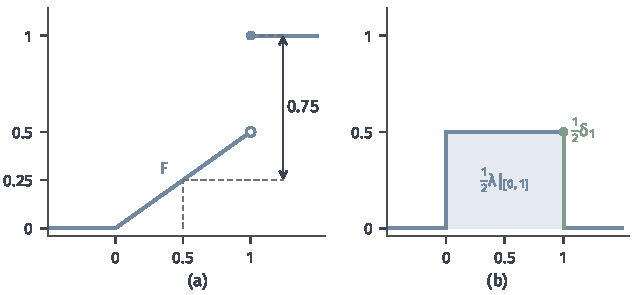
\includegraphics[width=108.000mm]{figures/04-spaces-measures-and-geometry/02-measure/matplotlib/meas-stieltjes-jump/figure.pdf}
  \caption{右连续单调函数$F$确定的Lebesgue--Stieltjes测度。(a)$F$在$[0,1)$上以斜率$1/2$增长，在$x=1$处跳跃$1/2$（实心点为$F(1)=1$，空心点为左极限$1/2$），竖向箭头是$(0.5,1]$的测度$0.75$；(b)$\mu_F$由总量$1/2$、均匀分布在$[0,1]$上的质量（蓝色密度$1/2$）与点质量$\frac12\delta_1$（绿色）组成。}
  \label{fig:meas-stieltjes-jump}
\end{BookInlineFigure}

\paragraph{Lebesgue测度}
取$F(x)=x$，得到$\mathcal B(\mathbb R)$上唯一满足$\lambda((a,b])=b-a$的测度$\lambda$。它没有点质量，所以开、闭、半开区间的测度都等于长度。

延拓定理的证明还给出更多信息。外测度$\lambda^*$由半开区间的可数覆盖定义，而每个半开区间$(a,b]$可以换成略长的开区间$(a,b+\varepsilon2^{-n})$，所以$\lambda^*$也等于用开区间覆盖的总长度的下确界，如图~\ref{fig:meas-outer-cover}所示。

\begin{BookInlineFigure}
  \centering
  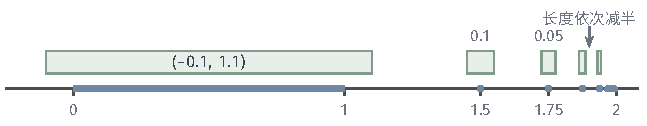
\includegraphics[width=109.552mm]{figures/04-spaces-measures-and-geometry/02-measure/tikz/meas-outer-cover/figure.pdf}
  \caption{用可数个开区间覆盖集合$E=[0,1]\cup\{1.5,1.75,1.875,\dots\}$（蓝色）。绿色区间是一种覆盖：$(-0.1,1.1)$盖住线段部分，长度依次减半的小区间盖住离散的点（只画出前几个）。这个覆盖的总长度为$1.2+0.1\cdot(1+\tfrac12+\tfrac14+\cdots)=1.4$；把各区间进一步缩短，总长度可以任意接近$1$，因此$\lambda^*(E)=1$。}
  \label{fig:meas-outer-cover}
\end{BookInlineFigure}

\begin{definition}[Lebesgue测度]
\label{def:meas-lebesgue}
关于$\lambda^*$为Carathéodory可测的全体集合称为\term{Lebesgue可测集}（Lebesgue measurable set），记作$\mathcal L$；$\lambda^*$在$\mathcal L$上的限制$\lambda$称为实轴上的\term{Lebesgue测度}（Lebesgue measure）。它在$\mathcal B(\mathbb R)$上的限制也称为Borel集上的Lebesgue测度，仍记作$\lambda$。
\end{definition}

覆盖平移后仍是覆盖，长度不变，所以$\lambda^*(E+t)=\lambda^*(E)$对一切$t\in\mathbb R$成立；判据~\eqref{eq:meas-caratheodory-criterion}中的等式随之平移，$\mathcal L$对平移封闭，Lebesgue测度具有平移不变性。

单点被$(x-\varepsilon,x+\varepsilon)$覆盖，测度为$0$，由可数次可加性，可数集的Lebesgue测度为$0$。回到有理点集：$\lambda(\mathbb Q\cap[0,1])=0$，$[0,1]$中无理数集合的测度为$1$。

同时，$[0,1]$是不可数个零测单点之并，整体测度却为$1$。这说明零测集的可数并仍零测，不可数并则不然。

\paragraph{Borel测度与它的完备化}
由Carathéodory定理，$(\mathbb R,\mathcal L,\lambda)$是完备的，且$\mathcal B(\mathbb R)\subseteq\mathcal L$。两者的差别恰好是零测集的子集，下面证明这一点。

设$E\in\mathcal L$且$\lambda(E)<+\infty$。按外测度的定义，对每个$n$有开区间列覆盖$E$且总长小于$\lambda(E)+1/n$，它们的并$U_n$是开集，$\lambda(U_n\setminus E)<1/n$。令$G=\bigcap_nU_n$，它是Borel集，满足
\[
 G\supseteq E,\qquad \lambda(G\setminus E)=0.
\]

对零测集$G\setminus E$再做一次同样的操作，得到Borel零测集$G'\supseteq G\setminus E$。于是
\[
 E=(G\setminus G')\cup(E\cap G'),
\]
第一项是Borel集，第二项包含于Borel零测集。无限测度的$E$切成可数个有限测度的片逐片处理即可。

反过来，$\mathcal L$完备且含$\mathcal B(\mathbb R)$，每个“Borel集并上Borel零测集的子集”都属于$\mathcal L$。所以$(\mathbb R,\mathcal L,\lambda)$正是$(\mathbb R,\mathcal B(\mathbb R),\lambda)$在定理~\ref{thm:meas-completion}意义下的完备化。

对一般的$F$，同样的构造给出$\mu_F$的完备化，它的可测集合族一般随$F$而变：$\mu_F=\delta_0$时，任何不含$0$的集合都是零测集的子集，完备化后全部子集都可测。所以“Borel测度”与“它的完备化”要分开说明，前者的可测范围固定为$\mathcal B(\mathbb R)$，后者的可测范围依赖测度本身。

\paragraph{Cantor集}
零测集是否一定可数？Cantor集给出否定的回答，后面它还会反复出现。

\begin{example}[Cantor集]
\label{ex:meas-cantor-set}
令$C_0=[0,1]$。把$C_{n-1}$中每个闭区间三等分，删去中间的开区间，得到$C_n$，它由$2^n$个长度为$3^{-n}$的闭区间组成，例如$C_1=[0,\tfrac13]\cup[\tfrac23,1]$。令
\[
 C=\bigcap_{n\geq0}C_n,
\]
称为\term{Cantor集}（Cantor set）。它是闭集的交，因而是闭集，也是Borel集。由$C\subseteq C_n$，
\[
 \lambda(C)\leq\lambda(C_n)=2^n\cdot3^{-n}=(2/3)^n\to0,
\]
所以$\lambda(C)=0$。

也可以从被删去的部分验算：第$n$步删去$2^{n-1}$个长度为$3^{-n}$的区间，总长度为
\[
 \sum_{n\geq1}\frac{2^{n-1}}{3^n}=\frac{1/3}{1-2/3}=1.
\]
被删去的总长度已经是$1$，留给$C$的长度只能是$0$。
\end{example}

图~\ref{fig:meas-cantor-set}画出了前四步。每一行的总长度按比例$2/3$缩小，同时区间的个数翻倍；留下的点集越来越稀，却始终非空。

\begin{BookInlineFigure}
  \centering
  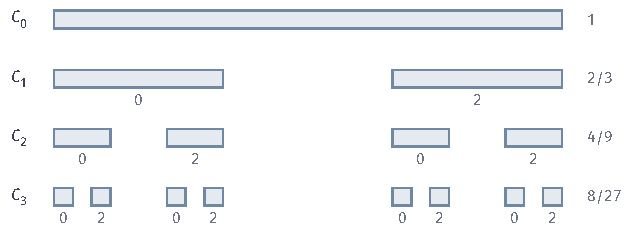
\includegraphics[width=107.142mm]{figures/04-spaces-measures-and-geometry/02-measure/tikz/meas-cantor-set/figure.pdf}
  \caption{Cantor集构造的前四步。第$n$行$C_n$由$2^n$个长度为$3^{-n}$的闭区间组成，右侧数字是总长度$(2/3)^n$；区间下方的三进制数字$0$或$2$记录这一步选择左段还是右段。}
  \label{fig:meas-cantor-set}
\end{BookInlineFigure}

Cantor集测度为零，却不可数。对每个$0$--$1$序列$s=(s_1,s_2,\dots)$，令
\[
 \phi(s)=\sum_{k\geq1}\frac{2s_k}{3^k},
\]
即三进制展开中只用数字$0$与$2$的数。前$n$位数字决定了前$n$步每一步选左段（数字$0$）还是右段（数字$2$），所以$\phi(s)\in C_n$对每个$n$成立，从而$\phi(s)\in C$。

$\phi$是单射。设$s\neq t$，第一个不同的位置为$k$，不妨$s_k=1$、$t_k=0$，则后面各项最多抵消$\sum_{j>k}2\cdot3^{-j}=3^{-k}$，于是
\[
 \phi(s)-\phi(t)\geq2\cdot3^{-k}-3^{-k}=3^{-k}>0.
\]
全体$0$--$1$序列不可数，故$C$不可数。零测性度量集合占据的长度，基数度量元素的多少，二者不能互相推出。

Cantor集还说明完备化确实增加了集合。$\lambda(C)=0$，由完备性，$C$的全部子集都Lebesgue可测，$C$与$\mathbb R$等势，所以这些子集和$\mathbb R$的全部子集一样多；而Borel集的个数只有连续统那么多，严格少于$\mathbb R$的子集个数。Borel集个数的证明要用到超限归纳，篇幅较长，读者可查阅\scite{math-folland1999real}。结论是：存在不是Borel集的Lebesgue可测集。

反过来，也存在不Lebesgue可测的集合。在$[0,1)$上规定$x\sim y$当且仅当$x-y\in\mathbb Q$，用选择公理从每个等价类选一个代表，组成集合$V$。令$\{r_k\}$为$[0,1)$中全体有理数，$V_k$为$V$按模$1$平移$r_k$的结果。这些$V_k$两两不交，并为$[0,1)$。

若$V$可测，平移不变性给出$\lambda(V_k)=\lambda(V)$，于是
\[
 1=\lambda([0,1))=\sum_k\lambda(V_k)=\sum_k\lambda(V).
\]
右边要么是$0$，要么是$+\infty$，不可能等于$1$。所以测度只能定义在某个$\sigma$代数上，不能假定全部子集都可测。

\paragraph{多维Lebesgue测度}
在$\mathbb R^d$上，把区间换成左开右闭矩形$\prod_{i=1}^d(a_i,b_i]$，长度换成体积。它们的有限不交并组成集合代数，体积在其上的可数可加性与一维相同：闭矩形是紧集，可数覆盖化为有限覆盖后，用全部矩形的边坐标把大矩形切成网格，逐块比较体积，就得到引理~\ref{lem:meas-finite-cover}的$d$维版本。

由延拓定理，得到$\mathcal B(\mathbb R^d)$上唯一满足$\lambda_d(R)=\lvert R\rvert$的测度$\lambda_d$，称为$d$维Lebesgue测度。它同样平移不变，其完备化的可测集称为$d$维Lebesgue可测集。$\lambda_d$与$d$个一维Lebesgue测度的乘积相同，这需要第~\ref{chap:integration}章的乘积测度来说明。

\section{有符号测度}
\label{sec:meas-signed}

测度只取非负值。可是很多量天然有正有负：一根杆上同时分布着正电荷与负电荷，一笔账在不同科目上有收入也有支出，两个概率分布在各个集合上的差有时为正、有时为负。最直接的模型是两个测度之差$\eta(A)=\nu(A)-\mu(A)$。本节研究这类赋值：它在哪里取正、在哪里取负，能否唯一地写回两个测度之差，以及怎样度量正负两方面的总量。积分尚未定义，本节只在集合层面讨论。

\subsection{正集与负集}
\label{sec:meas-positive-negative-sets}

\paragraph{从测度之差到有符号测度}
设$\nu,\mu$是$(X,\mathcal A)$上的测度，$\mu$有限。对两两不交的可测集$A_1,A_2,\dots$，两个测度各自可数可加，并且$\sum_n\mu(A_n)$收敛到有限值，所以
\[
 \eta\Bigl(\bigcup_nA_n\Bigr)=\sum_n\nu(A_n)-\sum_n\mu(A_n)=\sum_n\bigl(\nu(A_n)-\mu(A_n)\bigr)=\sum_n\eta(A_n).
\]
中间一步把两个级数逐项相减，这在至少一个级数有限时成立。可见$\eta=\nu-\mu$保留了可数可加性，只是不再非负；它可以取$+\infty$，但不会取$-\infty$。

两个无限测度不能直接相减。在$\mathbb N$上取计数测度$\nu$与$\mu=2\nu$，对无限集$A$，$\nu(A)-\mu(A)=+\infty-(+\infty)$没有定义。即使把它理解为某个数，也会和可数可加性冲突：$\mathbb N$分成单点后每块的差都是$-1$，级数和为$-\infty$；分成偶数集与奇数集后两块的差都没有定义。所以有符号测度必须禁止同时出现两种无穷。

\begin{definition}[有符号测度]
\label{def:meas-signed}
可测空间$(X,\mathcal A)$上的\term{有符号测度}（signed measure）是映射$\eta:\mathcal A\to[-\infty,+\infty]$，满足：$\eta$至多取$+\infty$与$-\infty$中的一个；$\eta(\varnothing)=0$；对任意两两不交的$A_1,A_2,\dots\in\mathcal A$，
\[
 \eta\Bigl(\bigcup_{n\geq1}A_n\Bigr)=\sum_{n\geq1}\eta(A_n),
\]
其中左端有限时，右端级数绝对收敛。若$\eta$只取有限实数值，称为\term{有限有符号测度}（finite signed measure）。
\end{definition}

“至多取一种无穷”保证了右端级数总有意义：各项中不会同时出现$+\infty$与$-\infty$。要求左端有限时级数绝对收敛，是因为不交集合的并与排列次序无关，右端也必须与次序无关；按实数级数的重排定理，这等价于绝对收敛。测度是有符号测度的特例，任意有限测度之差是有限有符号测度。

有符号测度是给\emph{集合}赋予实数的规则，不要与某些\emph{点}上取负值的函数混淆。$\eta(A)<0$表示集合$A$上的负质量多于正质量，这个数由整个集合决定。

\begin{example}[正负抵消]
\label{ex:meas-signed-weights}
取$X=\{1,2,3,4\}$及全部子集，规定单点值$\eta(\{1\})=2$，$\eta(\{2\})=-1$，$\eta(\{3\})=1$，$\eta(\{4\})=-2$，并令$\eta(A)=\sum_{i\in A}\eta(\{i\})$。它是有限有符号测度，也可以写成$\nu-\mu$，其中$\nu=2\delta_1+\delta_3$，$\mu=\delta_2+2\delta_4$。

计算几个值：$\eta(X)=2-1+1-2=0$，$\eta(\{1,2\})=1$，$\eta(\{1,3\})=3$，$\eta(\{2,4\})=-3$。全空间上的值为零只是正负抵消的结果；在$\{1,3\}$与$\{2,4\}$上，$\eta$的绝对值都达到$3$。所以$\eta(X)$很小甚至为零，不能说明$\eta$在各处都小。
\end{example}

例中的$\eta$还可以写成$(\nu+\delta_1)-(\mu+\delta_1)$。同一个有符号测度有许多种“测度减测度”的表示。我们要找的是由$\eta$本身确定、没有多余抵消的一种，第一步是找出$\eta$在哪里取正、在哪里取负。

\paragraph{正集与负集的定义}
只看$\eta(P)\geq0$并不够：例~\ref{ex:meas-signed-weights}中$\eta(\{1,2\})=1\geq0$，它的子集$\{2\}$却取$-1$。$\{1,2\}$整体为正，内部仍藏着负质量。要作为“正区域”，集合的每个可测部分都必须非负。

\begin{definition}[正集与负集]
\label{def:meas-positive-set}
设$\eta$是$(X,\mathcal A)$上的有符号测度。若$P\in\mathcal A$的每个可测子集$E$都满足$\eta(E)\geq0$，称$P$为$\eta$的\term{正集}（positive set）；若$N\in\mathcal A$的每个可测子集$E$都满足$\eta(E)\leq0$，称$N$为$\eta$的\term{负集}（negative set）。
\end{definition}

在例~\ref{ex:meas-signed-weights}中，$\{1,3\}$是正集，$\{2,4\}$是负集，$\{1,2\}$两者都不是。正集与负集可以同时是二者：$\eta$在其每个可测子集上都取零的集合，既是正集又是负集。

正集的可测子集仍是正集，可数个正集的并也是正集。若$P_1,P_2,\dots$是正集，$E\subseteq\bigcup_nP_n$可测，令$E_1=E\cap P_1$，$E_n=(E\cap P_n)\setminus(P_1\cup\dots\cup P_{n-1})$，则$E_n$是$P_n$的可测子集且两两不交，$\eta(E)=\sum_n\eta(E_n)\geq0$。负集同理。这两条封闭性是下面把正负区域拼起来的依据。

\subsection{Hahn分解与Jordan分解}
\label{sec:meas-hahn-jordan}

例~\ref{ex:meas-signed-weights}中，只要把$X$分成$\{1,3\}$与$\{2,4\}$，$\eta$在前一部分的每个子集上非负，在后一部分的每个子集上非正。一般的有符号测度是否也能一刀切成正、负两个区域？先对有限有符号测度证明，再说明扩展值的情形。

\paragraph{两条准备性质}
构造正负区域的思路是寻找使$\eta$最小的可测集。为此先要知道$\eta$的取值不会无限地向下延伸，并且单调集合列的连续性在有符号情形仍然成立。

\begin{lemma}[有限有符号测度有界]
\label{lem:meas-signed-bounded}
有限有符号测度$\eta$有界：存在$M<\infty$，使$\lvert\eta(A)\rvert\leq M$对一切$A\in\mathcal A$成立。
\end{lemma}

\begin{proof}
称可测集$A$是\emph{无界的}，如果$\sup\{\lvert\eta(E)\rvert:E\subseteq A,\ E\in\mathcal A\}=\infty$。设$X$是无界的，我们构造两两不交的可测集$B_1,B_2,\dots$，使每个$\lvert\eta(B_n)\rvert\geq1$。

设$A$无界。取可测子集$E\subseteq A$使$\lvert\eta(E)\rvert\geq\lvert\eta(A)\rvert+1$，则$\lvert\eta(A\setminus E)\rvert\geq\lvert\eta(E)\rvert-\lvert\eta(A)\rvert\geq1$。$E$与$A\setminus E$中至少有一个无界：否则$A$的任一可测子集$F$满足$\lvert\eta(F)\rvert\leq\lvert\eta(F\cap E)\rvert+\lvert\eta(F\setminus E)\rvert$，右边两项都有界。把无界的一块记为$A'$，另一块记为$B$，则$B\subseteq A\setminus A'$且$\lvert\eta(B)\rvert\geq1$。

从$A_0=X$出发反复执行这一步，得到无界集$A_0\supseteq A_1\supseteq\cdots$及$B_n\subseteq A_{n-1}\setminus A_n$，这些$B_n$两两不交。按定义~\ref{def:meas-signed}，$\sum_n\eta(B_n)$收敛到有限值$\eta(\bigcup_nB_n)$，通项必须趋于零，与$\lvert\eta(B_n)\rvert\geq1$矛盾。
\end{proof}

\begin{lemma}[有符号测度的单调连续性]
\label{lem:meas-signed-continuity}
设$\eta$是有限有符号测度。若$A_1\subseteq A_2\subseteq\cdots$，则$\eta(\bigcup_nA_n)=\lim_n\eta(A_n)$；若$A_1\supseteq A_2\supseteq\cdots$，则$\eta(\bigcap_nA_n)=\lim_n\eta(A_n)$。
\end{lemma}

\begin{proof}
对递增集合列，令$D_1=A_1$，$D_n=A_n\setminus A_{n-1}$，它们两两不交，$\bigcup_nA_n=\bigcup_nD_n$，部分和$\sum_{k\leq n}\eta(D_k)=\eta(A_n)$，由可数可加性得结论。对递减集合列，$A_1\setminus A_n$递增，并为$A_1\setminus\bigcap_nA_n$；由已证部分及$\eta(A_1\setminus B)=\eta(A_1)-\eta(B)$（各项有限），得$\eta(A_1)-\eta(\bigcap_nA_n)=\lim_n(\eta(A_1)-\eta(A_n))$。
\end{proof}

与测度不同，这里递减情形不需要另加有限性假设，因为$\eta$本身只取有限值。

\paragraph{Hahn分解}
若某个可测集$D$使$\eta$达到最小值，那么从$D$中拿走一个正值子集，或向$D$中添入一个负值的外部集合，都会让取值更小，这不可能；于是$D$是负集，补集是正集。难点在于证明最小值确实能被某个集合达到。

\begin{theorem}[Hahn分解]
\label{thm:meas-hahn}
设$\eta$是$(X,\mathcal A)$上的有符号测度。则存在$P\in\mathcal A$，使$P$是$\eta$的正集，$N=X\setminus P$是$\eta$的负集。这样的一对$(P,N)$称为$\eta$的\term{Hahn分解}（Hahn decomposition）。若$(P',N')$是另一组Hahn分解，则$P\cap N'$与$P'\cap N$的每个可测子集上$\eta$都取零。
\end{theorem}

\begin{proof}
先设$\eta$有限。令$m=\inf_{A\in\mathcal A}\eta(A)$。由引理~\ref{lem:meas-signed-bounded}，$m$是有限实数，又$\eta(\varnothing)=0$，故$m\leq0$。对每个$n$取可测集$A_n$使$\eta(A_n)<m+2^{-n}$。

第一步说明两个近乎最小的集合取交后仍近乎最小。对可测集$A,B$，有限可加性给出$\eta(A\cup B)+\eta(A\cap B)=\eta(A)+\eta(B)$；又$\eta(A\cup B)\geq m$，所以$\eta(A\cap B)\leq\eta(A)+\eta(B)-m$。固定$n$，对$k\geq n$令$C_{n,k}=A_n\cap\dots\cap A_k$，对$k$归纳得
\[
 \eta(C_{n,k+1})\leq\eta(C_{n,k})+\eta(A_{k+1})-m<m+\sum_{j=n}^{k+1}2^{-j}<m+2^{1-n}.
\]

第二步取极限。$C_{n,k}$关于$k$递减，令$C_n=\bigcap_{k\geq n}A_k$；由引理~\ref{lem:meas-signed-continuity}，$\eta(C_n)\leq m+2^{1-n}$。$C_n$关于$n$递增，令$D=\bigcup_nC_n$；再由该引理，$\eta(D)=\lim_n\eta(C_n)\leq m$。另一方面$\eta(D)\geq m$，所以$\eta(D)=m$，最小值被$D$达到。

第三步验证符号。若可测集$E\subseteq D$满足$\eta(E)>0$，则$\eta(D\setminus E)=m-\eta(E)<m$，矛盾，所以$D$是负集。若可测集$E\subseteq X\setminus D$满足$\eta(E)<0$，则$\eta(D\cup E)=m+\eta(E)<m$，同样矛盾，所以$X\setminus D$是正集。取$N=D$，$P=X\setminus D$即可。

对允许取一种无穷值的$\eta$，存在性的证明需要另一条引理：有限正值的集合中总能找到正值的正集。由此可以在正集中取使$\eta$接近上确界的一列，再用正集的可数并封闭性拼成最大的正区域。这里不给出这部分证明，可参考Folland的《Real Analysis》第3章。

最后看两组分解的差别，这一步对两种情形都适用。$P\cap N'$既是正集$P$的子集，又是负集$N'$的子集，它的每个可测子集$E$同时满足$\eta(E)\geq0$与$\eta(E)\leq0$，即$\eta(E)=0$。$P'\cap N$同理。
\end{proof}

Hahn分解一般不唯一：$\eta$在其上完全为零的区域可以划给任意一侧。在实轴上令$\eta=\lambda|_{[0,1]}-\lambda|_{[2,3]}$，$P_1=(-\infty,3/2)$与$P_2=(-\infty,2)$都给出Hahn分解，两者相差的$[3/2,2)$上$\eta$的每个子集都取零，见图~\ref{fig:meas-hahn-decomposition}。正区域还可以只差一个Lebesgue零测集，例如把点$1/2$从$P_1$移到负区域一侧。

\begin{figure}[!htbp]
  \centering
  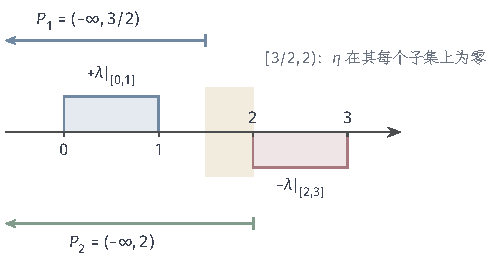
\includegraphics[width=84.06mm]{figures/02-abstract-mathematics/01-metric-and-measure/tikz/c2-hahn-decomposition/figure.pdf}
  \caption{Hahn分解的区域选择不唯一。$\eta=\lambda|_{[0,1]}-\lambda|_{[2,3]}$，蓝块在$[0,1]$上表示正的长度，红块在$[2,3]$上表示负的长度，块高表示长度测度前的系数$\pm1$。正区域可以取$P_1=(-\infty,3/2)$，也可以取$P_2=(-\infty,2)$；二者之差$[3/2,2)$（黄色）的每个可测子集上$\eta$都为零，所以放在哪一侧都不改变符号要求。}
  \label{fig:meas-hahn-decomposition}
\end{figure}

\paragraph{Jordan分解}
区域可以不同，限制在区域上的质量却是唯一的。把$\eta$分别限制到正区域与负区域，就得到两个测度。

\begin{theorem}[Jordan分解]
\label{thm:meas-jordan}
设$\eta$是有符号测度，$(P,N)$是它的一组Hahn分解。令
\[
 \eta^+(A)=\eta(A\cap P),\qquad \eta^-(A)=-\eta(A\cap N),\qquad A\in\mathcal A .
\]
则$\eta^+,\eta^-$是测度，其中至少一个有限，$\eta=\eta^+-\eta^-$，且$\eta^+(N)=\eta^-(P)=0$；它们不依赖于Hahn分解的选取。反过来，若$\eta=\alpha-\beta$，其中$\alpha,\beta$是测度、至少一个有限，并且存在可测集$S$使$\beta(S)=0$、$\alpha(X\setminus S)=0$，则$\alpha=\eta^+$，$\beta=\eta^-$。这个表示称为$\eta$的\term{Jordan分解}（Jordan decomposition），$\eta^+$、$\eta^-$分别称为$\eta$的\term{正变差}（positive variation）与\term{负变差}（negative variation）。
\end{theorem}

\begin{proof}
$A\cap P$是正集的子集，所以$\eta^+(A)\geq0$；同理$\eta^-(A)\geq0$。可数可加性直接来自$\eta$：若$A_n$两两不交，则$A_n\cap P$也两两不交。若$\eta$不取$+\infty$，则$\eta^+(X)=\eta(P)<+\infty$；若不取$-\infty$，则$\eta^-$有限。由$A=(A\cap P)\cup(A\cap N)$得$\eta(A)=\eta^+(A)-\eta^-(A)$，右边至多一项无穷，所以差有意义。$\eta^+(N)=\eta(\varnothing)=0$，$\eta^-(P)=0$。

再看与Hahn分解无关。设$(P',N')$是另一组分解。由定理~\ref{thm:meas-hahn}，$A\cap P\cap N'$与$A\cap P'\cap N$上$\eta$取零，因此
\[
 \eta(A\cap P)=\eta(A\cap P\cap P')+\eta(A\cap P\cap N')=\eta(A\cap P\cap P')=\eta(A\cap P'),
\]
最后一步对$P'$作同样的拆分。$\eta^-$同理。

最后证唯一性。设$\eta=\alpha-\beta$与$S$如定理所述。对$S$的可测子集$E$，$\eta(E)=\alpha(E)-0\geq0$；对$X\setminus S$的可测子集$E$，$\eta(E)=0-\beta(E)\leq0$。所以$(S,X\setminus S)$本身是一组Hahn分解。由已证的无关性，$\eta^+(A)=\eta(A\cap S)=\alpha(A\cap S)=\alpha(A)$，最后一步用了$\alpha(A\setminus S)=0$。同理$\beta=\eta^-$。
\end{proof}

定理中“存在$S$使$\beta(S)=0$、$\alpha(X\setminus S)=0$”说的是两个测度分别集中在两个不交的集合上，这种关系称为相互奇异，第~\ref{chap:measure-densities}章再系统比较。唯一性离不开这一条件。仍取$\eta=\lambda|_{[0,1]}-\lambda|_{[2,3]}$，它的Jordan分解是$\eta^+=\lambda|_{[0,1]}$、$\eta^-=\lambda|_{[2,3]}$。另一方面，令$\alpha=\lambda|_{[0,3]}$，$\beta=\lambda|_{[1,2]}+2\lambda|_{[2,3]}$，逐段检查系数：$[0,1]$上为$1-0$，$[1,2]$上为$1-1$，$[2,3]$上为$1-2$，所以同样有$\alpha-\beta=\eta$。但$\alpha,\beta$在$[1,3]$上重叠，总量都是$3$，而$\eta^\pm$的总量都是$1$。

这种多余的重叠只增不减。对任意表示$\eta=\alpha-\beta$（$\alpha,\beta$为测度，至少一个有限）及任意$A\in\mathcal A$，
\[
 \eta^+(A)=\eta(A\cap P)=\alpha(A\cap P)-\beta(A\cap P)\leq\alpha(A\cap P)\leq\alpha(A),
\]
同理$\eta^-(A)\leq\beta(A)$。所以Jordan分解是所有“测度减测度”表示中最小的一个。两种分解的输出不同：Hahn分解输出一个集合划分，它不唯一；Jordan分解输出两个测度，它唯一。

\subsection{全变差}
\label{sec:meas-total-variation}

$\lvert\eta(A)\rvert$衡量的是集合$A$上正负相抵后的净值，例~\ref{ex:meas-signed-weights}说明它可能掩盖很大的局部差别。要累计正负两方面的全部质量，应当把正变差与负变差相加，而不是相减。

\begin{definition}[全变差]
\label{def:meas-total-variation}
设$\eta$是有符号测度，$\eta=\eta^+-\eta^-$是它的Jordan分解。称测度
\[
 \lvert\eta\rvert=\eta^++\eta^-
\]
为$\eta$的\term{全变差测度}（total variation measure），称$\lvert\eta\rvert(X)$为$\eta$的\term{全变差}（total variation）。
\end{definition}

\paragraph{分割刻画}
$\lvert\eta\rvert$也可以不借助Jordan分解，直接从$\eta$的取值读出：把$A$切成有限块，对每块的净值取绝对值再相加。切得越合适，抵消越少；最合适的切法就是沿Hahn分解切开。

\begin{theorem}[全变差的分割刻画]
\label{thm:meas-total-variation-partition}
对每个$A\in\mathcal A$，
\[
 \lvert\eta\rvert(A)=\sup\Bigl\{\sum_{i=1}^k\lvert\eta(A_i)\rvert:\ k\geq1,\ A_1,\dots,A_k\in\mathcal A\text{两两不交},\ \bigcup_{i=1}^kA_i=A\Bigr\}.
\]
\end{theorem}

\begin{proof}
对$A$的任一有限可测分割，
\[
 \sum_i\lvert\eta(A_i)\rvert=\sum_i\lvert\eta^+(A_i)-\eta^-(A_i)\rvert\leq\sum_i\bigl(\eta^+(A_i)+\eta^-(A_i)\bigr)=\lvert\eta\rvert(A),
\]
所以上确界不超过$\lvert\eta\rvert(A)$。取Hahn分解$(P,N)$及分割$A_1=A\cap P$、$A_2=A\cap N$，则$\lvert\eta(A_1)\rvert+\lvert\eta(A_2)\rvert=\eta^+(A)+\eta^-(A)=\lvert\eta\rvert(A)$，上确界被达到。
\end{proof}

回到例~\ref{ex:meas-signed-weights}。不分割时$\lvert\eta(X)\rvert=0$；分成$\{1,2\}$与$\{3,4\}$时得$\lvert1\rvert+\lvert-1\rvert=2$；分成$\{1,3\}$与$\{2,4\}$时得$3+3=6$。再细分也不会超过$6$，因为四个单点上的绝对值之和为$2+1+1+2=6$。所以$\lvert\eta\rvert(X)=6$，正好由正负区域的分割取得，见图~\ref{fig:meas-total-variation-partition}。

\begin{figure}[!htbp]
  \centering
  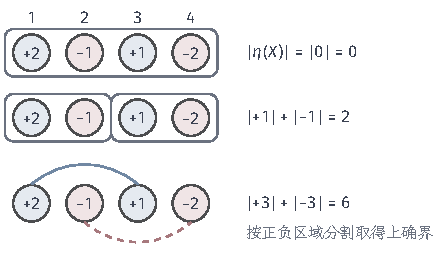
\includegraphics[width=75.128mm]{figures/02-abstract-mathematics/01-metric-and-measure/tikz/c2-total-variation-partition/figure.pdf}
  \caption{用分割读取全变差。四个点的权重为$+2,-1,+1,-2$。第一行不分割，净值为$0$；第二行把相邻的正负点合在一起，仍有抵消，绝对值之和为$2$；第三行按符号分组（蓝色实弧连接正点，红色虚弧连接负点），没有抵消，绝对值之和为$6=\lvert\eta\rvert(X)$。}
  \label{fig:meas-total-variation-partition}
\end{figure}

\paragraph{净值与总量}
由分割刻画取平凡分割$\{A\}$，立即得到$\lvert\eta(A)\rvert\leq\lvert\eta\rvert(A)$：左边允许抵消，右边累计正负变化的总量。特别地，$\lvert\eta\rvert(A)=0$当且仅当$\eta$在$A$的每个可测子集上都取零。所以$\lvert\eta\rvert$的零测集正是$\eta$完全看不见的集合；对有符号测度说“几乎处处”时，都相对于$\lvert\eta\rvert$来理解。

\paragraph{有限与扩展值两种情形}
若$\eta$是有限有符号测度，$\eta^+$与$\eta^-$都有限，$\lvert\eta\rvert$是有限测度，并且$\lvert\eta(A)\rvert\leq\lvert\eta\rvert(X)<\infty$对一切$A$成立，这与引理~\ref{lem:meas-signed-bounded}一致。若$\eta$取$+\infty$，则$\eta^+$无限而$\eta^-$有限，$\lvert\eta\rvert$在某些集合上为$+\infty$，此时只能在$\lvert\eta\rvert$有限的集合上作数值比较。

两个概率测度$P,Q$之差$\eta=P-Q$属于前一种情形。由$\eta(X)=0$得$\eta^+(X)=\eta^-(X)=\tfrac12\lvert\eta\rvert(X)$。又对每个可测集$A$有$\eta(A)\leq\eta^+(A)\leq\eta^+(X)$，取$A=P$时等号成立，所以
\[
 \tfrac12\lvert P-Q\rvert(X)=\eta^+(X)=\sup_{A\in\mathcal A}\bigl(P(A)-Q(A)\bigr).
\]
后续估计积分误差时，常用总量有限的$\lvert\eta\rvert$控制正负两方面的贡献；一个有符号测度何时能写成某个可积函数乘以参考测度，留到第~\ref{chap:measure-densities}章，那里同样要区分总量有限与允许扩展值的情形。

\section{可测映射}
\label{sec:meas-measurable-maps}

有了测度，下一步是把它用到函数上：一根细杆各处的线密度不同，总质量是多少；一个随机实验的结果被读成一个数，这个数落在某个区间里的概率是多少。每当对函数的输出提出“是否落在某集合中”的问题，就需要在输入端测量相应的点集。本节用原像刻画这一要求，先给出可测映射的定义与判据，再证明数值函数的常见运算和可数极限保持可测性，最后用只取有限个值的简单函数从下方逼近非负可测函数，为下一章定义积分准备对象。

\subsection{可测映射}
\label{sec:meas-measurable-map-def}

\paragraph{原像与可测性}
对映射$f:X\to Y$与$B\subseteq Y$，原像$f^{-1}(B)=\{x\in X:f(x)\in B\}$是“输出落在$B$中”的那些输入。原像对任意映射都有意义，并不要求$f$可逆。若输出端能提出的每个集合问题，在输入端都对应一个可测集合，就说$f$可测。

\begin{definition}[可测映射]
\label{def:meas-measurable-map}
设$(X,\mathcal A)$、$(Y,\mathcal B)$是可测空间。若对每个$B\in\mathcal B$都有$f^{-1}(B)\in\mathcal A$，称映射$f:X\to Y$为$\mathcal A/\mathcal B$-\term{可测映射}（measurable map），简称可测。
\end{definition}

可测性同时取决于两端的$\sigma$代数。在$X=\{1,2,3,4\}$上取由$\varnothing,\{1,2\},\{3,4\},X$组成的$\sigma$代数$\mathcal A$，在$Y=\{a,b\}$上取$\mathcal P(Y)$。令$f(1)=f(2)=a$、$f(3)=f(4)=b$，则$f^{-1}(\{a\})=\{1,2\}$、$f^{-1}(\{b\})=\{3,4\}$都可测，$f$可测。令$g(1)=a$、$g(2)=g(3)=g(4)=b$，则$g^{-1}(\{a\})=\{1\}\notin\mathcal A$，$g$不可测：输入端只知道点属于哪一组，无法回答“输出是否为$a$”。若把$Y$上的$\sigma$代数换成$\{\varnothing,Y\}$，$g$又变成可测的，因为输出端不再提出任何非平凡问题。

这与连续性的定义形式相同，内容不同。第~\ref{chap:topological-spaces}章的连续映射要求开集的原像是开集，可测映射要求可测集的原像是可测集。连续性关心邻近关系是否保持，可测性只关心集合问题能否在输入端回答，与距离和开集没有直接关系。

\paragraph{生成族判据}
直接检查$\mathcal B$中的每个集合往往做不到，例如$\mathcal B(\mathbb R)$中的集合无法逐一列出。原像与集合运算可交换，所以只需检查生成族。

\begin{lemma}[生成族判据]
\label{lem:meas-generator-criterion}
设$\mathcal B=\sigma(\mathcal C)$。若对每个$C\in\mathcal C$都有$f^{-1}(C)\in\mathcal A$，则$f$是$\mathcal A/\mathcal B$可测的。
\end{lemma}

\begin{proof}
令$\mathcal E=\{B\subseteq Y:f^{-1}(B)\in\mathcal A\}$。由$f^{-1}(Y)=X$、$f^{-1}(Y\setminus B)=X\setminus f^{-1}(B)$与$f^{-1}(\bigcup_nB_n)=\bigcup_nf^{-1}(B_n)$，$\mathcal E$是$Y$上的$\sigma$代数。它含$\mathcal C$，所以含$\sigma(\mathcal C)=\mathcal B$。
\end{proof}

由定义还可以直接得到复合规则。若$f:(X,\mathcal A)\to(Y,\mathcal B)$与$g:(Y,\mathcal B)\to(Z,\mathcal C)$都可测，则对$C\in\mathcal C$，$(g\circ f)^{-1}(C)=f^{-1}(g^{-1}(C))\in\mathcal A$，所以$g\circ f$可测。这里要求中间空间$Y$上两次使用的是同一个$\sigma$代数$\mathcal B$。

\paragraph{可测函数}
最常用的可测映射取实数值。目标端取$\mathcal B(\mathbb R)$；允许取$\pm\infty$时，在扩展实数$[-\infty,+\infty]$上取由$\mathcal B(\mathbb R)$与两个单点$\{-\infty\},\{+\infty\}$生成的$\sigma$代数。由定理~\ref{thm:meas-borel-generators}，半直线$(a,+\infty)$生成$\mathcal B(\mathbb R)$，再加上$\{+\infty\}=\bigcap_n(n,+\infty]$与$\{-\infty\}=[-\infty,+\infty]\setminus\bigcup_n(-n,+\infty]$，可知$(a,+\infty]$生成扩展实数上的这个$\sigma$代数。判据于是化为检查阈值集合。

\begin{definition}[可测函数]
\label{def:meas-measurable-function}
设$(X,\mathcal A)$是可测空间。若$f:X\to[-\infty,+\infty]$对每个$a\in\mathbb R$都有$\{f>a\}=\{x:f(x)>a\}\in\mathcal A$，称$f$为\term{可测函数}（measurable function）。当$(X,\mathcal A)=(\mathbb R^d,\mathcal B(\mathbb R^d))$时，称为\term{Borel可测函数}（Borel measurable function）。
\end{definition}

由生成族判据，实值函数$f$可测等价于它是$\mathcal A/\mathcal B(\mathbb R)$可测映射；只检查有理数$a$也够用。用补集与可数运算还可得到其他阈值集合，例如$\{f\geq a\}=\bigcap_n\{f>a-1/n\}$、$\{f\leq a\}=X\setminus\{f>a\}$，它们都可测。复值函数$f=u+\mathrm iv$称为可测，是指实部$u$与虚部$v$都可测。

集合的可测性与函数的可测性通过指示函数相连。对$A\subseteq X$，$\{\mathbf 1_A>a\}$在$a<0$时为$X$，在$0\leq a<1$时为$A$，在$a\geq1$时为$\varnothing$，所以$\mathbf 1_A$可测当且仅当$A\in\mathcal A$。例如$\mathbf 1_{\mathbb Q}$在$(\mathbb R,\mathcal B(\mathbb R))$上可测，因为$\mathbb Q$是Borel集；第~\ref{sec:meas-jordan}小节中它对应的集合连Jordan可测都不是。

\paragraph{连续映射与可测性}
设$X,Y$是度量空间，$f:X\to Y$连续。开集的原像是开集，因而属于$\mathcal B(X)$；开集生成$\mathcal B(Y)$，由生成族判据，$f$是$\mathcal B(X)/\mathcal B(Y)$可测的。所以连续函数都是Borel可测函数。

逆向结论不成立。阶跃函数$H=\mathbf 1_{[0,+\infty)}$的阈值集合是$\mathbb R$、$[0,+\infty)$或$\varnothing$，都是Borel集，所以$H$是Borel可测函数，但它在$0$处不连续；$\mathbf 1_{\mathbb Q}$处处不连续，却同样Borel可测。可测性只问阈值集合是否在允许测量的集合族里，对函数的局部变化没有任何要求。

上面的结论依赖两端都取Borel结构。若把两端都换成Lebesgue可测集$\mathcal L$，连续函数$f:\mathbb R\to\mathbb R$未必$\mathcal L/\mathcal L$可测：可以构造连续严格单调的$f$与零测集的子集$S$（由完备性，$S\in\mathcal L$），使$f^{-1}(S)$不Lebesgue可测。这里不展开构造，只记住：可测性必须写清两端的集合族，不能把目标端的Borel结构随意换成某个测度的完备化。本书中实值函数的目标端总取Borel结构。

\subsection{可测函数的运算}
\label{sec:meas-function-operations}

\paragraph{代数运算}
可测函数经过加、乘、取绝对值等运算后仍然可测。困难在于和的阈值集合$\{f+g>a\}$不能直接写成$f$与$g$各自阈值集合的有限组合，需要用有理数作可数分拆。

\begin{theorem}[可测函数的运算]
\label{thm:meas-function-operations}
设$f,g:X\to\mathbb R$可测，$c\in\mathbb R$，$\varphi:\mathbb R\to\mathbb R$连续。则$cf$、$f+g$、$\varphi\circ f$、$fg$、$\lvert f\rvert$、$\max\{f,g\}$、$\min\{f,g\}$都可测；若$g$处处不为零，$f/g$也可测。
\end{theorem}

\begin{proof}
$\varphi\circ f$是可测映射与Borel可测的连续函数之复合，所以可测。取$\varphi(t)=ct$、$\lvert t\rvert$、$t^2$，得$cf$、$\lvert f\rvert$、$f^2$可测。

对和，若$f(x)+g(x)>a$，则$f(x)>a-g(x)$，在两者之间取有理数$q$，有$f(x)>q$且$g(x)>a-q$；反之这两式蕴含$f(x)+g(x)>a$。所以
\[
 \{f+g>a\}=\bigcup_{q\in\mathbb Q}\bigl(\{f>q\}\cap\{g>a-q\}\bigr),
\]
是可数个可测集合之并。于是$f-g=f+(-1)g$可测。积由$fg=\tfrac14\bigl((f+g)^2-(f-g)^2\bigr)$得到，最大值与最小值由$\max\{f,g\}=\tfrac12(f+g+\lvert f-g\rvert)$与$\min\{f,g\}=\tfrac12(f+g-\lvert f-g\rvert)$得到。若$g$处处非零，$t\mapsto1/t$在$\mathbb R\setminus\{0\}$上连续，把它在$0$处任意赋值得到的Borel函数与$g$复合，可知$1/g$可测，从而$f/g$可测。
\end{proof}

复值可测函数按实部与虚部计算，同样对加法、乘法和取模封闭：$\lvert f\rvert=\sqrt{u^2+v^2}$是连续函数作用于$(u,v)$，可以先由$u^2+v^2$可测再取平方根。

\paragraph{扩展实值的运算范围}
允许取扩展实数值时，运算本身可能没有定义。$f+g$在$f(x)=+\infty$、$g(x)=-\infty$的点没有意义，必须先说明这样的点不出现，或者在那里另作约定；乘积还要约定$0\cdot(\pm\infty)$，本书取$0\cdot(\pm\infty)=0$。只有在这些点上的值确定以后，才能谈论运算结果是否可测。非负可测函数的和总有定义，并且可测：$\{f+g>a\}$在上式之外还要并上$\{f=+\infty\}\cup\{g=+\infty\}$。

\paragraph{函数列的上下确界与极限}
分析中的许多函数作为函数列的极限得到，例如级数的和与逐次逼近的结果。下一章的收敛定理正要处理这类极限，所以先确认极限对象仍然可测。

\begin{theorem}[可数极限的可测性]
\label{thm:meas-limits}
设$f_1,f_2,\dots:X\to[-\infty,+\infty]$可测。则$\sup_nf_n$、$\inf_nf_n$、$\limsup_nf_n$、$\liminf_nf_n$可测。若对每个$x$，极限$\lim_nf_n(x)$在$[-\infty,+\infty]$中存在，则极限函数可测。
\end{theorem}

\begin{proof}
$\sup_nf_n(x)>a$当且仅当某个$f_n(x)>a$，所以$\{\sup_nf_n>a\}=\bigcup_n\{f_n>a\}$可测。由$\inf_nf_n=-\sup_n(-f_n)$得下确界可测。上极限与下极限是可数次上、下确界的组合：
\[
 \limsup_{n\to\infty}f_n=\inf_{n\geq1}\sup_{k\geq n}f_k,\qquad \liminf_{n\to\infty}f_n=\sup_{n\geq1}\inf_{k\geq n}f_k,
\]
由前两步可测。极限存在时它等于上极限，因而可测。
\end{proof}

可数性在证明中不可缺少。设$S\subseteq\mathbb R$不是Borel集，对每个$s\in S$，$\mathbf 1_{\{s\}}$都是Borel可测函数，但它们的逐点上确界$\mathbf 1_S$不是，因为$\{\mathbf 1_S>0\}=S$。指标不可数时，$\{\sup_sf_s>a\}$是不可数并，$\sigma$代数不保证它可测。这个定理也只保证极限对象可测，不说明极限函数的积分等于积分的极限，那是下一章收敛定理的内容。

\paragraph{零测修改}
函数在零测集上的取值通常无关紧要，但修改后的函数是否仍然可测，取决于测度空间是否完备。设$f$可测，$g$与$f$只在某个零测集$N$内可能不同。若空间完备，则$\{g>a\}=(\{f>a\}\setminus N)\cup(\{g>a\}\cap N)$，第一项可测，第二项是零测集的子集，所以$g$可测。

若空间不完备，结论可能失败。在第~\ref{sec:meas-completion}小节的例子中，$X=\{1,2,3\}$，$\mathcal A=\{\varnothing,\{1\},\{2,3\},X\}$，$\mu=\delta_1$。取$f=0$、$g=\mathbf 1_{\{2\}}$，二者只在零测集$\{2,3\}$内不同，但$\{g>0\}=\{2\}$不可测。所以在一般测度空间中说“$g$与$f$几乎处处相等”时，要么先确认$g$可测，要么换到完备化空间上讨论。

\subsection{简单函数逼近}
\label{sec:meas-simple-approximation}

\paragraph{简单函数}
函数累计最容易的情形是函数只取有限个值：每个值占据一个可测集合，累计就是“值乘以集合的测度”再相加。这类函数是下一章定义积分的起点。

\begin{definition}[简单函数]
\label{def:meas-simple-function}
只取有限多个实数值的可测函数称为\term{简单函数}（simple function）。
\end{definition}

设简单函数$\varphi$的不同取值为$c_1,\dots,c_m$，令$A_i=\varphi^{-1}(\{c_i\})$。它们是可测集合，两两不交，并为$X$，于是
\begin{equation}
 \varphi=\sum_{i=1}^mc_i\mathbf 1_{A_i}.
 \label{eq:meas-simple-canonical}
\end{equation}
这称为$\varphi$的标准表示。反过来，任意可测集合$B_j$的有限线性组合$\sum_jb_j\mathbf 1_{B_j}$只取有限多个值，每个取值集合都是若干$B_j$及其补集之交的并，所以是简单函数。同一个简单函数可以有多种写法，例如$\mathbf 1_{[0,2]}=\mathbf 1_{[0,1]}+\mathbf 1_{(1,2]}$；下一章将说明积分不依赖于写法。简单函数的和、积、最大值仍是简单函数，因为结果仍只取有限个值。

\paragraph{按取值分层逼近}
怎样用简单函数逼近一般的非负可测函数？黎曼和的做法是把定义域切成小段，在每段上取一个高度；对一般的可测函数，定义域上可能没有任何一段使函数近似为常数，例如$\mathbf 1_{\mathbb Q}$。换一个方向：把值域切成小层，读出函数落在每一层的点集。这些点集是可测的，因为它们是函数的原像。

\begin{theorem}[简单函数逼近]
\label{thm:meas-simple-approximation}
设$f:X\to[0,+\infty]$可测。令
\begin{equation}
 \varphi_n=\sum_{k=0}^{n2^n-1}\frac k{2^n}\mathbf 1_{\{k2^{-n}\leq f<(k+1)2^{-n}\}}+n\,\mathbf 1_{\{f\geq n\}},\qquad n\geq1.
 \label{eq:meas-dyadic-approximation}
\end{equation}
则每个$\varphi_n$是非负简单函数，$0\leq\varphi_1\leq\varphi_2\leq\cdots\leq f$，并且$\varphi_n(x)\to f(x)$对每个$x\in X$成立。若$f$有界，收敛在$X$上是一致的。
\end{theorem}

\begin{proof}
各层$\{k2^{-n}\leq f<(k+1)2^{-n}\}$与$\{f\geq n\}$都是$f$的原像，可测，并且两两不交，所以$\varphi_n$是非负简单函数。按定义，$\varphi_n(x)$是把$\min\{f(x),n\}$向下取到$2^{-n}$的整数倍，于是$\varphi_n\leq f$。

单调性：从$n$到$n+1$，每一层$[k2^{-n},(k+1)2^{-n})$被分成两半，落在下半层的点取值不变，落在上半层的点取值增加$2^{-n-1}$；截断高度从$n$升到$n+1$，原来取值$n$的点只会取到不小于$n$的值。所以$\varphi_n\leq\varphi_{n+1}$。

收敛：若$f(x)<+\infty$，当$n>f(x)$时$0\leq f(x)-\varphi_n(x)<2^{-n}$，所以$\varphi_n(x)\to f(x)$。若$f(x)=+\infty$，则$\varphi_n(x)=n\to+\infty$。若$f\leq M$，当$n>M$时上面的误差估计对一切$x$同时成立，收敛是一致的。
\end{proof}

图~\ref{fig:meas-dyadic-approximation}以$[0,2]$上的$f(x)=x^2$为例画出了$\varphi_1$与$\varphi_2$。断点由函数值决定，而不是由定义域的等分决定：$\varphi_2$的断点在$x=\sqrt{k/4}$处，越靠近函数陡峭的地方越密。对一般的实值可测函数$f$，记$f^+=\max\{f,0\}$与$f^-=\max\{-f,0\}$，它们是非负可测函数，$f=f^+-f^-$，对两部分分别应用定理即得收敛到$f$的简单函数列，且$\lvert\varphi_n^+-\varphi_n^-\rvert\leq\lvert f\rvert$。

\begin{figure}[!htbp]
  \centering
  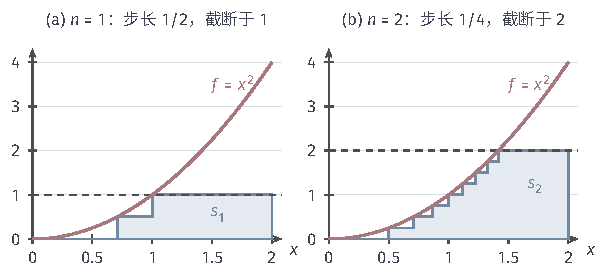
\includegraphics[width=102.634mm]{figures/02-abstract-mathematics/01-metric-and-measure/tikz/c3-dyadic-approximation/figure.pdf}
  \caption{二进分层逼近$f(x)=x^2$，$x\in[0,2]$。蓝色阶梯是$\varphi_n=2^{-n}\lfloor2^n\min\{f,n\}\rfloor$，虚线是截断高度$n$。(a)$n=1$，$\varphi_1$取值$0,0.5,1$；(b)$n=2$，$\varphi_2$取值$0,0.25,\dots,2$，断点为$\sqrt{k/4}$。阶梯始终位于曲线下方，且随$n$增大而升高。}
  \label{fig:meas-dyadic-approximation}
\end{figure}

这个逼近有三点要在下一章用到。第一，它从下方逼近，所以“下方简单函数的累计”自然成为非负函数积分的候选定义。第二，它单调递增，下一章将证明递增逼近的积分收敛到极限的积分。第三，它对每个非负可测函数都存在，不要求连续，也不要求有界；无界或取$+\infty$的函数由截断高度$n$逐步纳入。

\section{本章小结}
\label{sec:meas-summary}

本章开头问：区间里的有理点有多长，挖去无数个中间段后剩下的点集有多长，怎样把“分开测量、合起来相加”推广到这些集合。计数、长度与体积共有的是有限可加性，Jordan测量用有限个矩形从内外夹逼，能处理边界可以用有限个小矩形盖住的集合。有理点集的内外测量分别为$0$与$1$，暴露了有限覆盖的局限；改用可数覆盖，总长度可以任意小。

由此得到两项要求：允许测量的集合族对可数运算封闭，测量规则对可数不交分割可加。$\sigma$代数规定测量范围，生成$\sigma$代数只补入封闭性迫使加入的集合，度量空间的开集生成Borel集，实轴上的区间或半直线已经足够生成它。测度在$\sigma$代数上非负、可数可加，由此推出单调性、可数次可加性与从下连续性；从上连续性需要一个测度有限的起点。零测集与几乎处处说明哪些例外可以忽略，完备化补入零测集的子集而不改变原有集合的测度。

测度的构造分三步。外测度用可数覆盖的最小费用给每个子集赋值，但一般不可加；Carathéodory判据选出与外测度相容的集合，它们构成$\sigma$代数，外测度在其上可数可加。从集合代数上的预测度出发，这一路线给出延拓；延拓的唯一性另需$\sigma$有限条件，并由$\pi$--$\lambda$定理在生成族上比较。

对单调不减且右连续的$F$，区间增量$F(b)-F(a)$确定唯一的Stieltjes测度，跳跃给出点质量；取$F(x)=x$得到Lebesgue测度，它平移不变，其完备化正是Lebesgue可测集。Cantor集零测而不可数，说明测度与基数是两回事；不可测集的存在说明测度只能定义在某个$\sigma$代数上。

有符号测度允许正负值，但至多取一种无穷，以免出现无穷减无穷。Hahn分解把空间切成正集与负集，切法不唯一；Jordan分解把有符号测度写成两个分别集中在不交集合上的测度之差，这个表示唯一且最小。全变差$\lvert\eta\rvert=\eta^++\eta^-$累计正负两方面的质量，也等于有限分割上绝对值之和的上确界，它的零测集正是有符号测度完全看不见的集合。

可测映射用原像规定哪些函数可以用测度研究，只需在生成族上检查；实值函数的可测性归结为阈值集合可测。连续函数都Borel可测，反之不然。可测函数对代数运算和可数次上下确界、上下极限封闭，扩展实值的运算要先说明有定义的范围；零测修改是否保持可测性取决于完备性。

按取值分层得到的递增简单函数列从下方逼近每个非负可测函数，这是第~\ref{chap:integration}章定义积分的出发点。两个测度怎样比较、何时能写成参考测度的加权积分，留到第~\ref{chap:measure-densities}章；质量沿可测映射的转移留到第~\ref{chap:pushforward-measures}章。

